% Preambel mit Einstellungen importieren
% Document type and used packages
\documentclass[open=right, % Kapitel darf nur auf rechten Seite beginnen
    paper=A4,               % DIN-A4-Papier
    a4paper,                % DIN-A4-Papier
    12pt,                   % Schriftgöße
    headings=small,         % Kleine Überschriften
    headsepline=true,       % Trennlinie am Kopf der Seite
    footsepline=false,      % Keine Trennlinie am Fuß der Seite
    bibliography=totoc,     % Literaturverzeichnis in das Inhaltsverzeichnis aufnehmen
    twoside=on,             % Doppelseitiger Druck - auf off stellen für einseitig
    DIV=7,                  % Verhältnis der Ränder zum bedruckten Bereich
    chapterprefix=true,     % Kapitel x vor dem Kapitelnamen
    cleardoublepage=plain]{scrbook}

% Pakete einbinden, die benötigt werden
\usepackage{scrpage2}
\usepackage{subfigure}
\usepackage{float}
\usepackage{amsthm}
\usepackage[utf8]{inputenc}       % Dateien in UTF-8 benutzen
\usepackage[T1]{fontenc}          % Zeichenkodierung
\usepackage{graphicx}     % Bilder einbinden
\usepackage{gensymb}        % Degree Angaben
\usepackage[english, ngerman]{babel}       % Deutsch und Englisch unterstützen
\usepackage{xcolor}               % Color support
\usepackage{amsmath}              % Matheamtische Formeln
\usepackage{amsfonts}             % Mathematische Zeichensätze
\usepackage{amssymb}              % Mathematische Symbole
\usepackage{float}                % Fließende Objekte (Tabellen, Grafiken etc.)
\usepackage{booktabs}             % Korrekter Tabellensatz
\usepackage[printonlyused]{acronym}  % Abkürzungsverzeichnis [nur verwendete Abkürzugen]
\usepackage{makeidx}              % Sachregister
\usepackage{listings}             % Source Code listings
\usepackage{listingsutf8}         % Listings in UTF8
\usepackage[hang,font={sf,footnotesize},labelfont={footnotesize,bf}]{caption} % Beschriftungen
\usepackage[scaled]{helvet}     
\usepackage{caption}
\usepackage[absolute]{textpos}	  % Absolute Textpositionen (für Deckblatt)
\usepackage{calc}                 % Berechnung von Positionen
\usepackage{blindtext}            % Blindtexte
\usepackage[bottom=40mm,left=35mm,right=35mm,top=30mm]{geometry} % Ränder ändern
\usepackage{setspace}             % Abstände korrigieren
\usepackage{ifthen}               % Logische Bedingungen mit ifthenelse
\usepackage{scrhack}              % Get rid of tocbasic warnings
\usepackage[pagebackref=false,german]{hyperref}  % Hyperlinks
\usepackage[all]{hypcap}          % Korrekte Verlinkung von Floats
\usepackage[autostyle=true,german=quotes]{csquotes}   % Zitate
\usepackage[backend=biber,
  isbn=false,                     % ISBN nicht anzeigen, gleiches geht mit nahezu allen anderen Feldern
  %sortlocale=de_DE,               % Sortierung der Einträge für Deutsch
  sortlocale=en_US,              % Sortierung der Einträge für Englisch
  autocite=inline,                % regelt Aussehen für \autocite (inline=\parancite)
  hyperref=true,                  % Hyperlinks für Ziate
  style=ieee                     % Zitate als Zahlen [1]
  %style=alphabetic               % Zitate als Kürzel und Jahr [Ein05]
  %style=authoryear                % Zitate Author und Jahr [Einstein (1905)]
]{biblatex}                       % Literaturverwaltung mit BibLaTeX
\usepackage{rotating}             % Seiten drehen
\usepackage{harveyballs}          % Harveyballs

\setlength{\bibitemsep}{1em}     % Abstand zwischen den Literaturangaben
\setlength{\bibhang}{2em}        % Einzug nach jeweils erster Zeile

% Trennung von URLs im Literaturverzeichnis (große Werte [> 10000] verhindern die Trennung)
\defcounter{biburlnumpenalty}{10} % Strafe für Trennung in URL nach Zahl
\defcounter{biburlucpenalty}{500}  % Strafe für Trennung in URL nach Großbuchstaben
\defcounter{biburllcpenalty}{500}  % Strafe für Trennung in URL nach Kleinbuchstaben

% Farben definieren
\definecolor{linkblue}{RGB}{0, 0, 100}
\definecolor{linkblack}{RGB}{0, 0, 0}
\definecolor{comment}{RGB}{63, 127, 95}
\definecolor{darkgreen}{RGB}{14, 144, 102}
\definecolor{darkblue}{RGB}{0,0,168}
\definecolor{darkred}{RGB}{128,0,0}
\definecolor{javadoccomment}{RGB}{0,0,240}

% Einstellungen für das Hyperlink-Paket
\hypersetup{
    colorlinks=true,      % Farbige links verwenden
%    allcolors=linkblue,
    linktoc=all,          % Links im Inhaltsverzeichnis
    linkcolor=linkblack,  % Querverweise
    citecolor=linkblack,  % Literaturangaben
	filecolor=linkblack,  % Dateilinks
	urlcolor=linkblack    % URLs
}

% Einstellungen für Quelltexte
\lstset{
      xleftmargin=0.2cm,
      basicstyle=\footnotesize\ttfamily,
      keywordstyle=\color{darkgreen},
      identifierstyle=\color{darkblue},
      commentstyle=\color{comment},
      stringstyle=\color{darkred},
      tabsize=2,
      lineskip={2pt},
      columns=flexible,
      inputencoding=utf8,
      captionpos=b,
      breakautoindent=true,
	  breakindent=2em,
	  breaklines=true,
	  prebreak=,
	  postbreak=,
      numbers=none,
      numberstyle=\tiny,
      showspaces=false,      % Keine Leerzeichensymbole
      showtabs=false,        % Keine Tabsymbole
      showstringspaces=false,% Leerzeichen in Strings
      morecomment=[s][\color{javadoccomment}]{/**}{*/},
      literate={Ö}{{\"O}}1 {Ä}{{\"A}}1 {Ü}{{\"U}}1 {ß}{{\ss}}2 {ü}{{\"u}}1 {ä}{{\"a}}1 {ö}{{\"o}}1
}

\urlstyle{same}

% Einstellungen für Überschriften
\renewcommand*{\chapterformat}{%
  \Large\chapapp~\thechapter   % Große Schrift
  \vspace{0.3cm}               % Abstand zum Titel des Kapitels
}

% Abstände für die Überschriften setzen
\renewcommand{\chapterheadstartvskip}{\vspace*{2.6cm}}
\renewcommand{\chapterheadendvskip}{\vspace*{1.5cm}}

\RedeclareSectionCommand[
  beforeskip=-1.8\baselineskip,
  afterskip=0.25\baselineskip]{section}

\RedeclareSectionCommand[
  beforeskip=-1.8\baselineskip,
  afterskip=0.15\baselineskip]{subsection}

\RedeclareSectionCommand[
  beforeskip=-1.8\baselineskip,
  afterskip=0.15\baselineskip]{subsubsection}


% In der Kopfzeile nur die kurze Kapitelbezeichnung (ohne Kapitel davor)
\renewcommand*\chaptermarkformat{\thechapter\autodot\enskip}
\automark[chapter]{chapter}

% Einstellungen für Schriftarten
\setkomafont{pagehead}{\normalfont\sffamily}
\setkomafont{pagenumber}{\normalfont\sffamily}
\setkomafont{paragraph}{\sffamily\bfseries\small}
\setkomafont{subsubsection}{\sffamily\itshape\bfseries\small}
\addtokomafont{footnote}{\footnotesize}
\setkomafont{chapter}{\LARGE\selectfont\bfseries}

% Wichtige Abstände
\setlength{\parskip}{0.2cm}  % 2mm Abstand zwischen zwei Absätzen
\setlength{\parindent}{0mm}  % Absätze nicht einziehen
\clubpenalty = 10000         % Keine "Schusterjungen"
\widowpenalty = 10000        % Keine "Hurenkinder"
\displaywidowpenalty = 10000 % Keine "Hurenkinder"
\renewcommand{\footnotesize}{\fontsize{9}{10}\selectfont} % Größe der Fußnoten
\setlength{\footnotesep}{8pt} % Abstand zwischen den Fußnoten

% Index erzeugen
\makeindex

% Einfacher Font-Wechsel über dieses Makro
\newcommand{\changefont}[3]{
\fontfamily{#1} \fontseries{#2} \fontshape{#3} \selectfont}

% Eigenes Makro für Bilder
\newcommand{\bild}[3]{
\begin{figure}[h]
  \centering
  \includegraphics[width=#2]{#1}
  \caption{#3}
  \label{#1}
\end{figure}}

% Wo liegt Sourcecode?
\newcommand{\srcloc}{src/}
\newtheorem{mydef}{Definition}

% Wo sind die Bilder?
\graphicspath{{bilder/}}

% Makros für typographisch korrekte Abkürzungen
\newcommand{\zb}[0]{z.\,B.\ }
\newcommand{\dahe}[0]{d.\,h.\ }
\newcommand{\ua}[0]{u.\,a.\ }

% Flags für Veröffentlichung und Sperrvermerk
\newboolean{hsmapublizieren}
\newboolean{hsmasperrvermerk}


% Dokumenteninfos importieren
% -------------------------------------------------------
% Daten für die Arbeit
% Wenn hier alles korrekt eingetragen wurde, wird das Titelblatt
% automatisch generiert. D.h. die Datei titelblatt.tex muss nicht mehr
% angepasst werden.

\newcommand{\hsmasprache}{en} % de oder en für Deutsch oder Englisch
% Für korrekt sortierte Literatureinträge, noch preambel.tex anpassen
% und zwar bei \usepackage[main=ngerman, english]{babel},
% \usepackage[pagebackref=false,german]{hyperref}
% und \usepackage[autostyle=true,german=quotes]{csquotes}

% Titel der Arbeit auf Deutsch
\newcommand{\hsmatitelde}{Entwicklung von RFID Anwendungen zur Verwaltung von Beständen und Medikamenten in Krankenhäusern}

% Titel der Arbeit auf Englisch
\newcommand{\hsmatitelen}{Development of RFID applications for management and tracking assets and drugs in hospitals}

% Weitere Informationen zur Arbeit
\newcommand{\hsmaort}{Mannheim}    % Ort
\newcommand{\hsmaautorvname}{Jacqueline} % Vorname(n)
\newcommand{\hsmaautornname}{Franßen} % Nachname(n)
\newcommand{\hsmadatum}{31.08.2018} % Datum der Abgabe
\newcommand{\hsmajahr}{2018} % Jahr der Abgabe
\newcommand{\hsmafirma}{Escuela Politécnica de Ingeniería de Gijón} % Firma bei der die Arbeit durchgeführt wurde
\newcommand{\hsmabetreuer}{Prof. Dr. Miriam Föller-Nord, Hochschule Mannheim} % Betreuer an der Hochschule
\newcommand{\hsmazweitkorrektor}{Prof. Dr. Thomas Smits, Hochschule Mannheim} % Betreuer im Unternehmen oder Zweitkorrektor
\newcommand{\hsmafakultaet}{I} % I für Informatik
\newcommand{\hsmastudiengang}{IMB} % IB IMB UIB IM MTB

% Zustimmung zur Veröffentlichung
\setboolean{hsmapublizieren}{true}   % Einer Veröffentlichung wird zugestimmt
\setboolean{hsmasperrvermerk}{false} % Die Arbeit hat keinen Sperrvermerk

% -------------------------------------------------------
% Abstract

% Kurze (maximal halbseitige) Beschreibung, worum es in der Arbeit geht auf Deutsch
\newcommand{\hsmaabstractde}{Die folgende Bachelorthesis beschreibt die Entwicklung einer mobilen, hybriden Anwendung für Android- und iOS-Geräte. Das entwickelte System (Hardware und Software) zielt die Verfolgung und Verwaltung von medizinischen Geräten sowie Arzneimitteln in Krankenhäusern an.
Im Vergleich zu bisherigen Arbeiten behandelt die vorliegende Arbeit unter anderem die ''Real-time''-Synchronisierung, realisiert durch Socket.IO, zwischen Smartphones und dem Server im Krankenhaus. Dadurch wird ein möglichst synchroner Lösungsansatz verfolgt, um zeitnah auf etwaige Mängelbestände der Medikamente reagieren zu können.

Das vorliegende Projekt beabsichtigt die Entwicklung eines RFID basierten Systems für Verwaltungs- und Verfolgungsanwendungen. Insbesondere um die Kontrolle der Medikamenten, welche regelmäßig Patienten verabreicht werden, sowie medizinischer Geräte zu verbessern, soll das System in Krankenhäusern eingesetzt werden. Ein weiterer Benefit des vorgestellten System ist die Reduzierung 
von vergessener oder falscher Medikamentenverabreichung.
Das behandelte System besteht aus RFID Antennen, welche die Reichweite des Systems (in welcher RFID Tags erkannt werden) festlegen.
Diese Antennen und der RFID Leser sind verbunden mit einer Datenbank, welche Informationen zu den Gegenständen und Medikamenten enthält. Das Projekt deckt insbesondere Themen ab, die von großem Interesse für medizinische und ITC Firmen sind, wie beispielsweise Internet of Things und e-Health.}

% Kurze (maximal halbseitige) Beschreibung, worum es in der Arbeit geht auf Englisch

\newcommand{\hsmaabstracten}{The following Bachelor Thesis describes the on the development of a mobile hybrid application which can be run both on Android and iOS devices as well as the physical layer hardware based on RFID technology. The developed system (both hardware and software) is devoted to  be used for tracking and management of medical assets and drugs in hospitals. Compared to other existing systems, the given thesis includes the development of 'real-time' synchronization between client and server, realized by using Socket.IO. Thus, a very synchronous solution approach is pursued in order to react contemporarily to missing drugs.

This project aims to develop a RFID-based system for management and tracking applications. In particular, the proposed system is devoted to be deployed at hospitals, to ensure a better control of the medicines and medical tools that are periodically administered to the patients, reducing the probability of missed or wrong medicine administration. The proposed system is formed by a set of RFID antennas that will conform the coverage area where items tagged with RFID tags will be read. These antennas and the RFID reader will be connected to a database that will contain the information of the items to be monitored. The project covers topics of great interest for medical and ITC companies, such as IoT and e-Health.}


% Literatur-Datenbank
 % BibLaTeX-Datei mit Literaturquellen einbinden

\addbibresource{literatur.bib}   % BibLaTeX-Datei mit Literaturquellen einbinden

\begin{document}
\frontmatter

% Römische Ziffern für die "Front-Matter"
\setcounter{page}{0}
\changefont{ptm}{m}{n}  % Times New Roman für den Fließtext
\renewcommand{\rmdefault}{ptm}

% Titelblatt
% -------------------------------------------------------
% In dieser Datei sollten eigentlich keine Veränderungen mehr
% notwendig sein.
% -------------------------------------------------------

\thispagestyle{empty}

% Fakultäten der HS-Mannheim
% -------------------------------------------------------
\ifthenelse{\equal{\hsmafakultaet}{I}}%
  {\newcommand{\hsmafakultaetlangde}{Fakultät für Informatik}%
   \newcommand{\hsmafakultaetlangen}{Department of Computer Science}}{}

\ifthenelse{\equal{\hsmafakultaet}{E}}%
  {\newcommand{\hsmafakultaetlangde}{Fakultät für Elektrotechnik}%
   \newcommand{\hsmafakultaetlangen}{Department of Electrical Engineering}}{}

\ifthenelse{\equal{\hsmafakultaet}{S}}%
  {\newcommand{\hsmafakultaetlangde}{Fakultät für Sozialwesen}%
   \newcommand{\hsmafakultaetlangen}{Department of Social Work}}{}
   
\ifthenelse{\equal{\hsmafakultaet}{B}}%
  {\newcommand{\hsmafakultaetlangde}{Fakultät für Biotechnologie}%
   \newcommand{\hsmafakultaetlangen}{Department of Biotechnology}}{}

\ifthenelse{\equal{\hsmafakultaet}{D}}%
  {\newcommand{\hsmafakultaetlangde}{Fakultät für Gestaltung}%
   \newcommand{\hsmafakultaetlangen}{Department of Design}}{}

\ifthenelse{\equal{\hsmafakultaet}{M}}%
  {\newcommand{\hsmafakultaetlangde}{Fakultät für Maschinenbau}%
   \newcommand{\hsmafakultaetlangen}{Department of Mechanical Engineering}}{}

\ifthenelse{\equal{\hsmafakultaet}{N}}%
  {\newcommand{\hsmafakultaetlangde}{Fakultät für Informationstechnik}%
   \newcommand{\hsmafakultaetlangen}{Department of Information Technology}}{}
   
\ifthenelse{\equal{\hsmafakultaet}{W}}%
  {\newcommand{\hsmafakultaetlangde}{Fakultät für Wirtschaftsingenieurwesen}%
   \newcommand{\hsmafakultaetlangen}{Department of Engineering and Management}}{}
   
\ifthenelse{\equal{\hsmafakultaet}{C}}%
  {\newcommand{\hsmafakultaetlangde}{Fakultät für Verfahrens- und Chemietechnik}%
   \newcommand{\hsmafakultaetlangen}{Department of Chemical Process Engineering}}{}
   

\ifthenelse{\equal{\hsmastudiengang}{IB}}%
  {\newcommand{\hsmastudienganglangde}{Informatik}%
  \newcommand{\hsmastudienganglangen}{Computer Science}%
  \newcommand{\hsmatypde}{Bachelor-Thesis}%
  \newcommand{\hsmatypen}{Bachelor Thesis}%
  \newcommand{\hsmagrad}{\hsmabsc}}{}

\ifthenelse{\equal{\hsmastudiengang}{IMB}}%
  {\newcommand{\hsmastudienganglangde}{Medizinische Informatik}%
  \newcommand{\hsmastudienganglangen}{Medical Informatics}%
  \newcommand{\hsmatypde}{Bachelor-Thesis}%
  \newcommand{\hsmatypen}{Bachelor Thesis}%
  \newcommand{\hsmagrad}{\hsmabsc}}{}
  
\ifthenelse{\equal{\hsmastudiengang}{UIB}}%
  {\newcommand{\hsmastudienganglangde}{Unternehmens- und Wirtschaftsinformatik}%
  \newcommand{\hsmastudienganglangen}{Enterprise Computing}%  
  \newcommand{\hsmatypde}{Bachelor-Thesis}%
  \newcommand{\hsmatypen}{Bachelor Thesis}%
  \newcommand{\hsmagrad}{\hsmabsc}}{}

\ifthenelse{\equal{\hsmastudiengang}{IM}}%
  {\newcommand{\hsmastudienganglangde}{Informatik}%
   \newcommand{\hsmastudienganglangen}{Computer Science}%
   \newcommand{\hsmatypde}{Master-Thesis}%
   \newcommand{\hsmatypen}{Master Thesis}%
   \newcommand{\hsmagrad}{\hsmamaster}}{}

\ifthenelse{\equal{\hsmastudiengang}{MEB}}%
  {\newcommand{\hsmastudienganglangde}{Mechatronik}%
   \newcommand{\hsmastudienganglangen}{Mechatronic}%
   \newcommand{\hsmatypde}{Bachelor-Thesis}%
   \newcommand{\hsmatypen}{Bachelor Thesis}%
   \newcommand{\hsmagrad}{\hsmabsc}}{}
   
\ifthenelse{\equal{\hsmastudiengang}{UB}}%
  {\newcommand{\hsmastudienganglangde}{Automatisierungstechnik}%
   \newcommand{\hsmastudienganglangen}{Automation Technology}%
   \newcommand{\hsmatypde}{Bachelor-Thesis}%
   \newcommand{\hsmatypen}{Bachelor Thesis}%
   \newcommand{\hsmagrad}{\hsmabsc}}{}
   
\ifthenelse{\equal{\hsmastudiengang}{ELB}}%
  {\newcommand{\hsmastudienganglangde}{Elektro- und Informationstechnik/Ingenieurpädagogik}%
   \newcommand{\hsmastudienganglangen}{Elektro- und Informationstechnik/Ingenieurpädagogik}%
   \newcommand{\hsmatypde}{Bachelor-Thesis}%
   \newcommand{\hsmatypen}{Bachelor Thesis}%
   \newcommand{\hsmagrad}{\hsmabsc}}{} 
   
\ifthenelse{\equal{\hsmastudiengang}{EBE}}%
  {\newcommand{\hsmastudienganglangde}{Energietechnik und erneuerbare Energien}%
   \newcommand{\hsmastudienganglangen}{Power Engineering ans Renewable Energies}%
   \newcommand{\hsmatypde}{Bachelor-Thesis}%
   \newcommand{\hsmatypen}{Bachelor Thesis}%
   \newcommand{\hsmagrad}{\hsmabsc}}{}

\ifthenelse{\equal{\hsmastudiengang}{TS}}%
  {\newcommand{\hsmastudienganglangde}{Translation Studies}%
   \newcommand{\hsmastudienganglangen}{Translation Studies}%
   \newcommand{\hsmatypde}{Bachelor-Thesis}%
   \newcommand{\hsmatypen}{Bachelor Thesis}%
   \newcommand{\hsmagrad}{\hsmabsc}}{}
  
\ifthenelse{\equal{\hsmastudiengang}{EM}}%
  {\newcommand{\hsmastudienganglangde}{Automatisierungs- und Energiesysteme}%
   \newcommand{\hsmastudienganglangen}{Automation and Energy Systems}%
   \newcommand{\hsmatypde}{Master-Thesis}%
   \newcommand{\hsmatypen}{Master Thesis}%
   \newcommand{\hsmagrad}{\hsmamaster}}{}
   
\ifthenelse{\equal{\hsmastudiengang}{ELM}}%
  {\newcommand{\hsmastudienganglangde}{Lehramt Ingenieurpädagogik}%
   \newcommand{\hsmastudienganglangen}{Lectureship Educational Engineering}%
   \newcommand{\hsmatypde}{Master-Thesis}%
   \newcommand{\hsmatypen}{Master Thesis}%
   \newcommand{\hsmagrad}{\hsmamaster}}{}
   
\ifthenelse{\equal{\hsmastudiengang}{SAB}}%
  {\newcommand{\hsmastudienganglangde}{Soziale Arbeit}%
   \newcommand{\hsmastudienganglangen}{Social Labour}%
   \newcommand{\hsmatypde}{Bachelor-Thesis}%
   \newcommand{\hsmatypen}{Bachelor Thesis}%
   \newcommand{\hsmagrad}{\hsmaba}}{}
   
\ifthenelse{\equal{\hsmastudiengang}{SAM}}%
  {\newcommand{\hsmastudienganglangde}{Soziale Arbeit}%
   \newcommand{\hsmastudienganglangen}{Social Labour}%
   \newcommand{\hsmatypde}{Master-Thesis}%
   \newcommand{\hsmatypen}{Master Thesis}%
   \newcommand{\hsmagrad}{\hsmamastera}}{}
   
\ifthenelse{\equal{\hsmastudiengang}{BB}}%
  {\newcommand{\hsmastudienganglangde}{Biotechnology}%
   \newcommand{\hsmastudienganglangen}{Biotechnology}%
   \newcommand{\hsmatypde}{Bachelor-Thesis}%
   \newcommand{\hsmatypen}{Bachelor Thesis}%
   \newcommand{\hsmagrad}{\hsmabsc}}{}
   
\ifthenelse{\equal{\hsmastudiengang}{BCB}}%
  {\newcommand{\hsmastudienganglangde}{Biologische Chemie}%
   \newcommand{\hsmastudienganglangen}{Biological Chemics}%
   \newcommand{\hsmatypde}{Bachelor-Thesis}%
   \newcommand{\hsmatypen}{Bachelor Thesis}%
   \newcommand{\hsmagrad}{\hsmabsc}}{}
   
\ifthenelse{\equal{\hsmastudiengang}{BMEBST}}%
  {\newcommand{\hsmastudienganglangde}{Biotechnology - Biomedical Science and Technology}%
   \newcommand{\hsmastudienganglangen}{Biotechnology - Biomedical Science and Technology}%
   \newcommand{\hsmatypde}{Master-Thesis}%
   \newcommand{\hsmatypen}{Master Thesis}%
   \newcommand{\hsmagrad}{\hsmamaster}}{}
   
\ifthenelse{\equal{\hsmastudiengang}{BMEBPD}}%
  {\newcommand{\hsmastudienganglangde}{Biotechnology - Bioprocess Development}%
   \newcommand{\hsmastudienganglangen}{Biotechnology - Bioprocess Development}%
   \newcommand{\hsmatypde}{Master-Thesis}%
   \newcommand{\hsmatypen}{Master Thesis}%
   \newcommand{\hsmagrad}{\hsmamaster}}{}
   
\ifthenelse{\equal{\hsmastudiengang}{BLSM}}%
  {\newcommand{\hsmastudienganglangde}{Life Science Management}%
   \newcommand{\hsmastudienganglangen}{Life Science Management}%
   \newcommand{\hsmatypde}{Master-Thesis}%
   \newcommand{\hsmatypen}{Master Thesis}%
   \newcommand{\hsmagrad}{\hsmamaster}}{}
   
\ifthenelse{\equal{\hsmastudiengang}{KDB}}%
  {\newcommand{\hsmastudienganglangde}{Kommunikationsdesign}%
   \newcommand{\hsmastudienganglangen}{Communication Design}%
   \newcommand{\hsmatypde}{Bachelor-Thesis}%
   \newcommand{\hsmatypen}{Bachelor Thesis}%
   \newcommand{\hsmagrad}{\hsmaba}}{}
   
\ifthenelse{\equal{\hsmastudiengang}{KDM}}%
  {\newcommand{\hsmastudienganglangde}{Kommunikationsdesign}%
   \newcommand{\hsmastudienganglangen}{Communication Design}%
   \newcommand{\hsmatypde}{Master-Thesis}%
   \newcommand{\hsmatypen}{Master Thesis}%
   \newcommand{\hsmagrad}{\hsmamastera}}{}
   
\ifthenelse{\equal{\hsmastudiengang}{MB}}%
  {\newcommand{\hsmastudienganglangde}{Maschinenbau}%
   \newcommand{\hsmastudienganglangen}{Mechanical Engineering}%
   \newcommand{\hsmatypde}{Bachelor-Thesis}%
   \newcommand{\hsmatypen}{Bachelor Thesis}%
   \newcommand{\hsmagrad}{\hsmabsc}}{}
   
\ifthenelse{\equal{\hsmastudiengang}{MM}}%
  {\newcommand{\hsmastudienganglangde}{Maschinenbau}%
   \newcommand{\hsmastudienganglangen}{Mechanical Engineering}%
   \newcommand{\hsmatypde}{Master-Thesis}%
   \newcommand{\hsmatypen}{Master Thesis}%
   \newcommand{\hsmagrad}{\hsmamaster}}{}
   
\ifthenelse{\equal{\hsmastudiengang}{NEB}}%
  {\newcommand{\hsmastudienganglangde}{Elektronik}%
   \newcommand{\hsmastudienganglangen}{Electronics}%
   \newcommand{\hsmatypde}{Bachelor-Thesis}%
   \newcommand{\hsmatypen}{Bachelor Thesis}%
   \newcommand{\hsmagrad}{\hsmabsc}}{}
   
\ifthenelse{\equal{\hsmastudiengang}{TIB}}%
  {\newcommand{\hsmastudienganglangde}{Technische Informatik}%
   \newcommand{\hsmastudienganglangen}{Technical Information Technology}%
   \newcommand{\hsmatypde}{Bachelor-Thesis}%
   \newcommand{\hsmatypen}{Bachelor Thesis}%
   \newcommand{\hsmagrad}{\hsmabsc}}{}
   
\ifthenelse{\equal{\hsmastudiengang}{MTB}}%
  {\newcommand{\hsmastudienganglangde}{Medizintechnik}%
   \newcommand{\hsmastudienganglangen}{Medical Technology}%
   \newcommand{\hsmatypde}{Bachelor-Thesis}%
   \newcommand{\hsmatypen}{Bachelor Thesis}%
   \newcommand{\hsmagrad}{\hsmabsc}}{}
   
\ifthenelse{\equal{\hsmastudiengang}{MTM}}%
  {\newcommand{\hsmastudienganglangde}{Medizintechnik}%
   \newcommand{\hsmastudienganglangen}{Medical Technology}%
   \newcommand{\hsmatypde}{Master-Thesis}%
   \newcommand{\hsmatypen}{Master Thesis}%
   \newcommand{\hsmagrad}{\hsmamaster}}{}
   
\ifthenelse{\equal{\hsmastudiengang}{NM}}%
  {\newcommand{\hsmastudienganglangde}{Informationstechnik}%
   \newcommand{\hsmastudienganglangen}{Informationstechnik}%
   \newcommand{\hsmatypde}{Master-Thesis}%
   \newcommand{\hsmatypen}{Master Thesis}%
   \newcommand{\hsmagrad}{\hsmamaster}}{}
   
\ifthenelse{\equal{\hsmastudiengang}{WB}}%
  {\newcommand{\hsmastudienganglangde}{Wirtschaftsingenieurwesen}%
   \newcommand{\hsmastudienganglangen}{Business Administration and Engineering}%
   \newcommand{\hsmatypde}{Bachelor-Thesis}%
   \newcommand{\hsmatypen}{Bachelor Thesis}%
   \newcommand{\hsmagrad}{\hsmabsc}}{}
   
\ifthenelse{\equal{\hsmastudiengang}{WM}}%
  {\newcommand{\hsmastudienganglangde}{Wirtschaftsingenieurwesen}%
   \newcommand{\hsmastudienganglangen}{Business Administration and Engineering}%
   \newcommand{\hsmatypde}{Master-Thesis}%
   \newcommand{\hsmatypen}{Master Thesis}%
   \newcommand{\hsmagrad}{\hsmamaster}}{}
   
\ifthenelse{\equal{\hsmastudiengang}{VB}}%
  {\newcommand{\hsmastudienganglangde}{Verfahrenstechnik}%
   \newcommand{\hsmastudienganglangen}{Process Engineering}%
   \newcommand{\hsmatypde}{Bachelor-Thesis}%
   \newcommand{\hsmatypen}{Bachelor Thesis}%
   \newcommand{\hsmagrad}{\hsmabsc}}{}
   
\ifthenelse{\equal{\hsmastudiengang}{CB}}%
  {\newcommand{\hsmastudienganglangde}{Chemische Technik}%
   \newcommand{\hsmastudienganglangen}{Chemical Engineering}%
   \newcommand{\hsmatypde}{Bachelor-Thesis}%
   \newcommand{\hsmatypen}{Bachelor Thesis}%
   \newcommand{\hsmagrad}{\hsmabsc}}{}
   
\ifthenelse{\equal{\hsmastudiengang}{CM}}%
  {\newcommand{\hsmastudienganglangde}{Chemieingenieurwesen}%
   \newcommand{\hsmastudienganglangen}{Chemical Engineering}%
   \newcommand{\hsmatypde}{Master-Thesis}%
   \newcommand{\hsmatypen}{Master Thesis}%
   \newcommand{\hsmagrad}{\hsmamaster}}{}

\newcommand{\hsmabsc}{Bachelor of Science (B.Sc.)}
\newcommand{\hsmaba}{Bachelor of Arts (B.A.)}
\newcommand{\hsmamaster}{Master of Science (M.Sc.)}
\newcommand{\hsmamastera}{Master of Arts (M.A.)}
\newcommand{\hsmamasterba}{Master of Business Administration (MBA)}

\newcommand{\hsmakoerperschaftde}{Hochschule Mannheim}
\newcommand{\hsmakoerperschaften}{University of Applied Sciences Mannheim}

\newcommand{\hsmaautorbib}{\hsmaautornname, \hsmaautorvname} % Autor Nachname, Vorname
\newcommand{\hsmaautor}{\hsmaautorvname \ \hsmaautornname} % Autor Vorname Nachname

\ifthenelse{\equal{\hsmasprache}{de}}%
  {\newcommand{\hsmatyp}{\hsmatypde}%
   \newcommand{\hsmathesistype}{zur Erlangung des akademischen Grades \hsmagrad}%
   \newcommand{\hsmakoerperschaft}{\hsmakoerperschaftde}%
   \newcommand{\hsmastudiengangname}{Studiengang \hsmastudienganglangde}%
   \newcommand{\hsmastudienganglang}{\hsmastudienganglangde}%
   \newcommand{\hsmatitel}{\hsmatitelde}%
   \newcommand{\hsmatutor}{Betreuer}%
   \newcommand{\hsmafakultaetlang}{\hsmafakultaetlangde}%
   \newcommand{\hsmalistoftables}{Tabellenverzeichnis}%
   \newcommand{\hsmalistoffigures}{Abbildungsverzeichnis}%
   \newcommand{\hsmalistings}{Quellcodeverzeichnis}%
   \newcommand{\hsmaindex}{Index}%
   \newcommand{\hsmaabbreviations}{Abkürzungsverzeichnis}%   
   \selectlanguage{ngerman}}%
  {\newcommand{\hsmatyp}{\hsmatypen}%
   \newcommand{\hsmathesistype}{for the acquisition of the academic degree \hsmagrad}%
   \newcommand{\hsmakoerperschaft}{\hsmakoerperschaften}%
   \newcommand{\hsmastudiengangname}{Course of Studies: \hsmastudienganglang}%
   \newcommand{\hsmastudienganglang}{\hsmastudienganglangen}%
   \newcommand{\hsmatitel}{\hsmatitelen}%
   \newcommand{\hsmatutor}{Tutors}
   \newcommand{\hsmafakultaetlang}{\hsmafakultaetlangen}%
   \newcommand{\hsmalistoftables}{List of Tables}%
   \newcommand{\hsmalistoffigures}{List of Figures}%
   \newcommand{\hsmalistings}{Listings}%
   \newcommand{\hsmaindex}{Index}%
   \newcommand{\hsmaabbreviations}{List of Abbreviations}%
   \selectlanguage{english}}%


% Daten in die Standard-Felder von KOMA-Script eintragen
\titlehead{\hsmatyp\ in\  \hsmastudienganglang}
\subject{}
\title{\hsmatitel}
\author{\hsmaauthor}
\date{\small{\hsmadatum}}

% Daten für das fertige PDF-Dokument
\hypersetup{
  pdftitle={\hsmatitel},  % Titel des Dokuments
  pdfauthor={\hsmaautor},              % Autor
  pdfsubject={\hsmatyp\ in\ \hsmastudienganglang},                % Thema
  pdfkeywords={\hsmatitel}         % Schlüsselworte
}

\newlength{\bindekorrektur}
\newlength{\seitenanfang}
\newlength{\seitenbreite}
  
\setlength{\bindekorrektur}{-46mm}   % Korrektur der horizontalen Position
\setlength{\seitenanfang}{0mm}       % Korrektur der vertikalen Position
\setlength{\seitenbreite}{297mm}

\noindent
\includegraphics[width=7cm]{hsma-logo.pdf}\\

% Titel der Arbeit
\begin{textblock*}{128mm}(45mm,\seitenanfang + 62mm) % 4,5cm vom linken Rand und 6,0cm vom oberen Rand
  \centering\Large\sffamily
  \vspace{4mm} % Kleiner zusätzlicher Abstand oben für bessere Optik
  \textbf{\hsmatitel}
\end{textblock*}%

% Name
\begin{textblock*}{128mm}(45mm,\seitenanfang + 103mm)
  \centering\large\sffamily
  \hsmaautor
\end{textblock*}

% Thesis
\begin{textblock*}{\seitenbreite}(\bindekorrektur,\seitenanfang + 130mm)
  \centering\large\sffamily
  \hsmatyp\\
  \begin{small}\hsmathesistype \end{small}\\
  \vspace{2mm}
  \hsmastudiengangname
\end{textblock*}

% Fakultät
\begin{textblock*}{\seitenbreite}(\bindekorrektur,\seitenanfang + 165mm)
  \centering\large\sffamily
  \hsmafakultaetlang\\
  \vspace{2mm}
  \hsmakoerperschaft
\end{textblock*}

% Datum
\begin{textblock*}{\seitenbreite}(\bindekorrektur,\seitenanfang + 190mm)
  \centering\large 
  \textsf{\hsmadatum}
\end{textblock*}

% Firma
\begin{textblock*}{\seitenbreite}(\bindekorrektur,\seitenanfang + 215mm)
  \centering\large 
  %\textsf{Durchgeführt bei der Firma \hsmafirma}
\end{textblock*}

% Betreuer
\begin{textblock*}{\seitenbreite}(\bindekorrektur,\seitenanfang + 240mm)
  \centering\large\sffamily
  \hsmatutor \\
  \vspace{2mm}
  \hsmabetreuer\\
  \vspace{2mm}
  \hsmazweitkorrektor
\end{textblock*}

% Bibliographische Informationen
\null\newpage
\thispagestyle{empty}
  
\newcommand{\hsmabibde}{\begin{small}\textbf{\hsmaautorbib}: \\ \hsmatitelde \ / \hsmaautor. \ -- \\ \hsmatypde, \hsmaort : \hsmakoerperschaftde, \hsmajahr. \pageref{lastpage} Seiten.\end{small}}

\newcommand{\hsmabiben}{\begin{small}\textbf{\hsmaautorbib}: \\ \hsmatitelen \ / \hsmaautor. \ -- \\ \hsmatypen, \hsmaort : \hsmakoerperschaften, \hsmajahr. \pageref{lastpage} pages. \end{small}}

\ifthenelse{\equal{\hsmasprache}{de}}%
  {\hsmabibde \\ \vspace{0.5cm} \\ \hsmabiben}
  {\hsmabiben \\ \vspace{0.5cm} \\ \hsmabibde}


% Erklärung
\clearpage\setcounter{page}{1}
\thispagestyle{empty}
\textsf{\large\textbf{Erklärung}}

Hiermit erkläre ich, dass ich die vorliegende Arbeit selbstständig verfasst und keine anderen als die angegebenen Quellen und Hilfsmittel benutzt habe.

\ifthenelse{\boolean{hsmapublizieren} \and \not\boolean{hsmasperrvermerk}}%
{
\vspace{0.5cm}
Ich bin damit einverstanden, dass meine Arbeit veröffentlicht wird, d.\,h. dass die Arbeit elektronisch gespeichert, in andere Formate konvertiert, auf den Servern der Hochschule Mannheim öffentlich zugänglich gemacht und über das Internet verbreitet werden darf. 
}{}%


\vspace{1cm}
\hsmaort, \hsmadatum \\

\vspace{1.2cm}						                                      
\hsmaautor

\ifthenelse{\boolean{hsmasperrvermerk}}%
{%
\vspace{11cm}
\color{red}\textsf{\large\textbf{Sperrvermerk}}

Diese Arbeit basiert auf internen und vertraulichen Daten des Unternehmens \hsmafirma.

Diese Arbeit darf Dritten, mit Ausnahme der betreuenden Dozenten und befugten Mitglieder des Prüfungsausschusses, ohne ausdrückliche Zustimmung des Unternehmens und des Verfassers nicht zugänglich gemacht werden.

Eine Vervielfältigung und Veröffentlichung der Arbeit ohne ausdrückliche Genehmigung -- auch in Auszügen -- ist nicht erlaubt.
\color{black}
}{}

\cleardoublepage

% Abstract
\chapter*{Abstract}

\ifthenelse{\equal{\hsmasprache}{de}}%
  {\subsubsection*{\hsmatitelde}\hsmaabstractde\subsubsection*{\hsmatitelen}\hsmaabstracten}
  {\subsubsection*{\hsmatitelen}\hsmaabstracten\subsubsection*{\hsmatitelde}\hsmaabstractde}


% Inhaltsverzeichnis erzeugen
\cleardoublepage
\pdfbookmark{\contentsname}{Contents}
\tableofcontents

% Korrigiert Nummerierung bei mehrseitigem Inhaltsverzeichnis
\cleardoublepage
\newcounter{frontmatterpage}
\setcounter{frontmatterpage}{\value{page}}

% Arabische Zahlen für den Hauptteil
\mainmatter

% Den Hauptteil mit vergrößertem Zeilenabstand setzen
\onehalfspacing

% ------------------------------------------------------------------
% Hauptteil der Arbeit
\chapter{Use of RFID Technology}
\label{Kap1}

The following chapter will discuss the reasons why choosing the technology and the scope of the RFID technology. It will start by explaining fundamental information and functionalities of RFID readers, tags and further equipment to build a RFID application. After that, some 'State of the Art' applications and use cases will be shown. In the end, there will be mentioned some large companies which provide medical RFID solutions.

\section{Motivation}

Concerning the organization and management of medical devices or patients in a hospital, there exist many problems. In the following, some examples of these problems as described by Ajami and Rajabzadeh \cite{ncbi} will be given.

\subsection{Decision Making}

First of all, when it comes to decision making, e.g. about the correct treatment of a severe illness, many physicians are stumped for an answer or their opinions are divided. To enable a rapid diagnosis and to improve the patient's health status, 'smart healthcare' \cite{henrici} would help a lot. For instance, RFID tags which are equipped with sensors to ensure the effectiveness of medicine accelerate the treatment process a lot. Furthermore, patients or hospital beds equipped with RFID tags make it easier to identify and manage the amount of patients as well as the workflow.

\subsection{Internal Communication}

Secondly, poor communication between nurses and physicians deteriorates medical supply. For instance, if a nurse notices that a patient needs a more tranquilizer because he became very nervous, she has to tell the doctor to dose the patient with the correct amount of tranquilizer. But often, a physician is occupying another patient. So, the communication is one problem but the other problem is the staff shortage. Thus, inadequate patient monitoring is emerges. And sometimes, there is the risk of misidentification of patients. To explain the last point, there is an easy example: At the urology department are two elder patients, Paul Schmitt and Jochen Schmitt. They are not brothers or related to each other and suffer from different types of illness. Paul suffers from kidney insufficiency whereas Jochen suffers from prostatic lithiasis. The first one needs a dialysis every day whereas the second one needs a radiosurgery. Because both patients are unable to walk themselves, nurses and clinical staff have to bring them to the particular treatment room. The problem should be easy to understand, both patients have the same surname but need completely different treatments. If the treatments would be commuted, their health status would deteriorate and they might die because of the misidentification.

\subsection{Investment possibilities}

Another important point for hospitals is the budget and their possibilities to investigate in new technologies which makes the enrollment of a new RFID system more challenging. Furthermore, clinical staff and phycisians have to be introduced into the new technologies. Not only the human factor plays a significant role but also the existing systems, such as the \ac{HIS}, \ac{RIS} or \ac{LIS}. If a new identifying system or software should be integrated into a hospital or healthcare institution, it has to be deployed suitably to the existing system architecture. To achieve the last point, Ajami and Rajabzadeh \cite{ncbi} recommend starting with small RFID projects and mentions countermeasures to increase the acceptance of such applications by healthcare institutions. To give an example, the regulations to protect patient's privacy should be mature to achieve more institutional support. Besides, there should exist more customized RFID systems which accomplish the individual tasks of their users.  

\subsection{Medication Administration System}

To explain the positive impact of using RFID systems, in the following, a few applications will be described briefly (see also \cite{ncbi}). Firstly, Ajami and Rajabzadeh describe a Medication Administration System which automatically verifies medication and generates the corresponding medication medicine. There exists multiple intents of developing a Administration System, such as preventing human errors (like for example mislabeling of tissue specimens in gastrointestinal and colorectal surgery endoscopy units). The second most common error which occured were that patients have been labelled incorrectly. To avoid these errors, an initiative of developing an application of RFID technology to specimen bottles was started. The aim of this initiative was to create a paperless pathology requisition system and the correct confirmation by both the endoscopy nursing staff as well as the endoscopist for each specimen bottle. As a result of deploying the application, specimen-labeling errors were significantly reduced.

\subsection{Wisely Aware RFID Dosage}

Another RFID system, called \ac{WARD} system should prevent the risk of medication errors triggered by medical staff. It is based on integrated barcode and RFID tags which should demonstrate effective and safe patient care environment. 
To give another example of RFID applications, the following paragraph will describe the \ac{MIMS} which includes a mobile nursing care system using RFID technology. There are many implemented functionalities in the MIMS, such as the tracking of patient's vital signs across various locations and in different medical facilities. The vital sign monitoring enables medical staff to watch critical ill patients carefully and permanently and reduces the risk of serious harm resulting from slow provision \cite{ncbi}. The mobile application MIMS offers alarming services in case of emergencies and can always be taken everywhere. Behind the frontend, a rule-based clinical decision supports medical staff and the mobile nursing environment. Last but not least, MIMS has been extended to most medical domains and has been integrated with other HIS.

\subsection{RFID applications in hospitals: A case study}

In their conference paper, Wang et al. \cite{casestudy} describe a case study of implementing a RFID system in a Taiwan hospital in the year 2003. The project that was studied was named \ac{LBMS} and was performed in the \ac{TMUH}. In the following section, the development strategy, device management as well as the value generation which are important for developing RFID applications in healthcare organizations, will be discussed. 
Referring to a widely spread disease, called \ac{SARS} in 2003, the authors Wang et al. discuss the effectiveness of applying RFID in hospitals to prevent further infections (e.g. of patients or medical staff). They mention several challenges of implementing RFID systems in hospitals, for instance user/physician resistance, investment problems as well as technical, clinical, organizational and professional resistance. Nevertheless, some hospitals initiated (with subsidies from the Taiwanese government) preliminary RFID projects as early as October 2003 and achieved significant results. 

To give a basic introduction into the existing IT infrastructure in the TMUH, the following paragraph will mention the existing systems of the hospital. TMUH has an integrated HIS that complies with several healthcare standards, such as \ac{HL7}, \ac{DICOM} \cite[p.3 ff.]{casestudy}. Furthermore, the system consists of a LIS, RIS and according to Wang et al. most of the patient's medical records are digitalized. When it comes to the development and the reasons for using LBMS, the authors wanted to build a system that could detect and track potential SARS cases. Medical knowledge and practice should form the basis and core for developing the system. The RFID technology was considered as a tool to support medical practice. In the end, the system should reflect medical assumptions. 
Wang et al. describe a basic workflow with four steps of the LBMS: Initially, all data should be stored in a positioning database which is connected to the existing vital information databases (of the HIS). In the second step, the system automatically retrieves patient medical records from the HIS and runs an inference engine (called 'Rulebase').  'Rulebase' judges whether there was an infectious event or not. If there was a infectious event, the system detects this in a third step. As a consequence (step four) of the detected event, a message is sent immediately to relevant personnel via alarm (email and sms). 
The LBMS can be extended and used in other contexts, like e.g. for precious equipment tracing, in-patient medicine auditing, new-born baby and mother identification or legitimate drug control.
Wang et al. were supported by the Taiwanese government which approved their plan and granted money. As the LBMS should be released as a hospital-wide system, the development required expertise and knowledge from different domains, including medicine, RFID technology, IT systems development, telecommunications and systems integration. Actually, three parties were involved: TMUH, Lion Information Inc. and an advisory group \cite[p.4]{casestudy} which consisted of professors emerging technology and making academic contributions (algorithms).
Since the hospital decided that the system should have active real-time position-tracking, temperature taking and monitoring abilities for tagged patients, the developing team chose 916,5 MHz UHF active tags (see Chapter 2, RFID tags \pageref{tag}) to reduce the risk of staff infections.

Reaching an adequate system integration without loss of performance, functionality and security was a big challenge. With the use of a field generator, a small tag wake-up device that communicates directly with the reader, the real-time communication should be realized \cite[p.4]{casestudy}. The generator periodically turns on and calls tags for a specific time. There exist three different types of generators: Normal, floor and area generators.
Furthermore, Wang et al. bring up the challenge of the entire device management \cite[p.5]{casestudy} with the purpose of collecting and transmitting reads that are as complete and clean as possible. Realizing a complete device management was limited by compartments, rooms, walls and doors because of their buildling layouts and materials which interfere with radiowaves. Besides, the balance between accuracy requirements and investment costs has to be maintained. Moreover, unauthorized removal of tags has to be managed carefully, since there might be some patients who try to take off their RFID wristband. In this case, an additional alarm has to be designed. All in all, the design and deployment of RFID devices depend on the environment and the context in which they are used. 
Not only the device management was challenging but also the data management as Wang et al. mention. The authors describe two general problems of data management in their RFID system. On the one hand, there occur intermittent and unreliable reads. These might be compensated by developing algorithms to process missing and incomplete reads. On the other hand, there will be generated high-volume data in a very short time. To prohibit this, the data should be filtered by algorithms and only the necessary data should be transmitted. For instance, if a tagged patient exceeded the present degree of 0.5°C, his data would be transmitted. To come to a conclusion, data management is tied to medical knowledge and practices which can substantially reduce the volume of data to be handled. As a result, meaningful information for decision making will be generated.
 
Besides the LBMS project \cite[p.2 ff.]{casestudy}, Wang et al. depict some existing RFID applications. To give an example of a succesful use of RFID, the U.S. Department of Defence has been using the technology for years. 
To give an overview of the usual hospital applications until 2006, Wang et al. depict applications for tracking and managing equipment such as wheelchairs, portable heart monitors. Moreover, trials on tagging patients, staff and equipment in rooms were conducted in several hospitals. Besides, the Washington Hospital Center (Washington D.C.) deployed a RFID system to track the status and the exact location of patients, staff as well as the essential equipment.
During the realization of the mentioned projects, the solutions depended on building an RFID infrastructure together with the middleware and the impedance-matching of the RFID system and the current systems (e.g. \ac{ERP} systems). Actually, to get along with the mentioned solutions, a strong team work (involving people from IT and business departments) and project management should be included. 
Since RFID allows wireless storage and automatic retrieval of data, there exists an 'ecosystem' of companies trying to develop a platform to support RFID development and applications.  Besides the variety of existing systems in hospitals, Wang et al. mention three mayor technical challenges accomplishing a RFID system. First, the non-line-of-sight reading might be a challenge since there exist various types of tags and the frequencies influence the range of signal. Second, handling of serial numbers might be a challenge which could be coped with setting a primary key to each tag which synchronizes with an existing database (see Chapter 3, 'Used platforms and technologies' \pageref{platforms}. The third challenge is to deal with the real-time data and to synchronize it seasonably. To deal with the third challenge, the use of NoSQL databases makes sense and will be discussed in Chapter 3 \pageref{nosql}.

Finally, Wang et al. evaluate RFID as an infrastructure technology which allows companies to capture data about objects and individuals moving in the real world \cite[p.7]{casestudy}. In addition to that, the authors claim that organizations should think carefully how to change business processes to reap the benefits of RFID. By naming benefits of RFID, Wang et al. refer to the improved efficiency, patient safety and reduced medical errors which can be very extensive and expensive nowadays \cite{casestudy}.

\section{Aim and Scope}

Ajami and Rajabzadeh \cite{ncbi} mention three important purposes of RFID technology. The first purpose of using RFID is to improve the tracking of objects. It is mainly used to follow products through a specific supply chain or to follow medical devices an drugs in the clinical workflow. There is also the possibility to track a product to a particular patient or to identify clinicians who administered medication to patients.
The second purpose for which RFID technology is appropriate is the inventory management (see section \pageref{inventory}). Inventory Management is significant for managing an organization, like a hospital. There are many complex processes where information about the location, time and the amount of material is necessary (e.g. towels, duvet covers).
The third and last purpose of RFID technology, mentioned by Ajami and Rajabzadeh \cite{ncbi}, is validation. Using RFID to identify and validate data is an effective method for ensuring the quality of a hospital or healthcare setting. It ensures that the patient being treated is the right patient.

uhf, reaching signal -->see chapter \chapterref{Kap2}







 % Externe Datei einbinden

\chapter{General Information about RFID technology}
\label{Kap2}

\section{General Information}

According to Ajami and Rajabzadeh \cite{ncbi} RFID technology is capable of an automatic unambiguous identifiation without being placed in the line of sight of their objects. The data between RFID tags and readers is transmitted through radio waves. In the 1940ies, the technology was firstly used to identify airplanes during war. Today, it is used in several different areas, like for example in manufacturing, supply chains, agriculture, transportation systems, healthcare services etc. 

\subsection{Components of an RFID application}

Ajami and Rajabzadeh \cite{ncbi} mention five main components existing in a RFID system. Firstly, there is the RFID tag attached to an object ensuring its unique identification. Secondly, the has to be an antenna which detects each tag and creates a magnetic field. The antenna is connected to its reader which receives the tag's information and is able to manipulate tags. Thirdly, in every RFID system has to exist a communication infrastructure which enables the interaction of readers and tags through an \ac{IT} infrastructure. Lastly, to enable users to connect to the RFID infrastructure and to control its modules, there has to be established a application software, such as a database or user interface.

\subsubsection{RFID tags} \label{tags}

Henrici \cite{henrici} states that there are two types of RFID tags: Tags with 'Smartcard'-like functionality and 'Auto-id' systems. The first type of RFID tag  provides extended functionalities and has computational capabilities. Furthermore, sensors can be attached to the 'Smartcard'-like tags which measure and control temperature and can be used for telemetry applications. In contrast, the 'Auto-id' systems imply the automatic identification of its objects. Generally spoken, RFID systems can be seen as a subset of 'Auto-id' systems.

When it comes to the variety of RFID tags, three fundamental types are distinguished: Active, semi-active and passive RFID tags \cite{henrici} which all constist of an antenna, a microchip and packaging. Active RFID tags consist of a microchip and have their own power source. As a characteristic, they are more expensive than the other two types. After that, semi-active tags or also called 'hybride' tags have their own power supply which is only used to support the microchip. The transmission or communication between semi-active tag and reader is implemented by using the power of the reader's field. Lastly, the passive RFID tags do not consist of a power source and only work in the reading range of the reader. They harvest their needed energy from the electromagnetic field of the reader and are cheaper than active tags. Moreover, passive tags are lighter than active tags and provide a long-lasting service. In constrast to active tags, passive tags are limited in their read range and functionality.

According to Henrici \cite{henrici}, the memory capacity of passive RFID tags can vary from single bits to kilobytes which is not much. As a recommendation, an external database to store tag-specific data should be used. For instance, a memory of 12 byte is very common to store \ac{EPC}. Concerning the memory technology, Henrici distinguishes two general types of storage: non-volatile and volatile storage. Non-volatile storage can be divided into read-only (fixed after manufacturing), \ac{WORM} and read-write which set the access privileges to the memory. The opposite of non-volatile storage is called volatile storage and is used for example to perform calculations after power-up. Besides, Henrici mentions tags which check passwords or implement ciphering algorithms to ensure data privacy. To visualize the tag's data and to provide real-time measurement, passive tags can be equipped with displays, buttons and temperature sensors. 

To maintain the security and authenticity of each RFID tag, Henrici \cite[p.93 ff.]{henrici} depicts four implementation methods of identification. 
The first and easiest method is called 'regular identification'. It implies that each tag sends its complete identifier to the reader within a \ac{SMLE}. Another method is called 'implicit identification'. It uses information that has not been provided explicitly for particular identification purpose. Thirdly, a more complexe and secure method to identify tags which is called 'multistep identification' is described by Henrici. As the name of this method is very self-explaining, one has to think of three identification steps: In the first step, only parts of the identification information is revealed. After that, an authentication and authorization step follows. Once, being authenticated and authorized, more identification information will be revealed. 
Other than the mentioned methods, Henrici describes a fourth and most secure method to identify tags which he calls 'encryption and shared key identification'. As an advantage, this identification method protects every information contained in an identifier which can be transmitted in encrypted form. The vast amount of information requires a high internal storage of the tag, like given by active tags. To arrange an encrypted tranmission of information from passive, low cost tags the identifier needs to be calculated outside the tag and then stored on the tag (directly in enciphered form). So, it would be no additional expenditure to enable encrypted and shared key identification of tags using passive tags. 

\begin{figure}
\centering
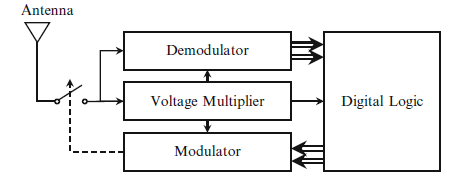
\includegraphics[width=\textwidth]{rfidtagdesign} The design of RFID tags 
\caption{\label{fig:tagdesign}The adopted from \cite[p.13]{chipless}} 
\end{figure}

\subsubsection{RFID readers} \label{reader}

In this section, RFID readers will be explained in detail. To start with, one has to imagine existing objects which are tagged with a RFID tag. To implement functionality to these tags and to connect them to a middleware or a backend system, a detector is needed. This detector is the RFID reader and consists of an antenna, a power supply for passive tags, a microprocessor (to control devices) and an interface for forwarding data to the processing backend system \cite{henrici}. 
Generally, two different types of readers can be distinguished: Stationary and mobile readers. To give an example of the use of stationary readers, they can be used for goods receiving or stock management. Furthermore, stationary readers are fixed to a specific location and need permanent network connection. On the opposite, mobile readers do not need permanent network connection and are used for querying prices in a supermarket.
As mentioned in the section before \pageref{tags}, RFID tags and readers communicate via electromagnetism. The reader's detection range depends on the frequency as well as the electromagnetic field \cite{henrici}. In general, four frequency ranges can be differenced: \ac{LF} (125-134 kHz),\ac{HF}(13,56 MHz), \ac{UHF} (868 MHz-915 MHz) and Microwave (2,54 GHz-5,8 GHz). Each frequency range has its own physical characteristics, such as the needed size of antennas or the read range.
According to Vizinex \cite{vizinex}, an american company with site in Pennsylvania, U.S HF tags can be used for short read ranges (up to 3 inches). They are usually tagged to tissue samples, blood and critical fluids. Furthermore, HF tags work well in proximidity to liquids as well as human tissues. UHF tags provide longer read ranges and can be detuned by proximity to tissue, fluids and metals. These tags are typically used to track and locate critical medical devices, manage inventories of medical items and track as well as identify patients. Moreover, UHF tags are compatible with worldwide standards and easily deployed because of the compatibility with widely available and competitively priced RFID readers.
Furthermore, each reader has its own electromagnetic field. Such fields are distinguished into near field and far fields: Near fields, also called magnetic or electric fields work with induction and capacitive coupling whereas far fields consist of electromagnetic waves. The measuring unit of electromagnetic fields is called field strength and the maximal field strength depends on national regulations. These national regulations limit the electromagnetic compatibility to avoid disturbing other systems. The functionality of passive tags within near field is different from passive tags in far field. In near field, the tags send data to the reader using load modulation. This mechanism does not work in far fields: Here, the sended frequency is backscattered \cite{henrici}.
All in all, readers are able to query tags and to read and write tag data. But the storage of information and the information processing does not take place in readers or tags, but in the middleware or backend systems. These will be explained in the following paragraph.

\begin{figure}
\centering
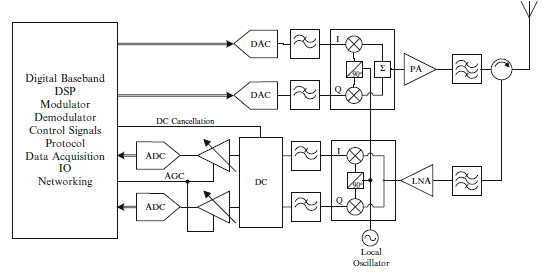
\includegraphics[width=\textwidth]{rfidreaderdesign} The design of a RFID reader 
\caption{\label{fig:readerdesign}The adopted from \cite[p.17]{chipless}} 
\end{figure}

\subsubsection{RFID backend systems} \label{backend}

As Henrici \cite{henrici} mentions, the backend can be divided into two parts: Middleware and applications. Both of them run on the same computer within the same network which is important for the permanent connection to RFID readers and all existing tags. The advantages of a middleware in this use are that no adaption of appications is needed, an open and neutral interface for other applications is provided. Besides, as the middleware is used to aggregate and filter data the processing is moved from tags into middleware so that tags only have to identify objects. As a result, modularity of the system is maintained.

Concerning the data management of RFID systems, data is barely stored on RFID tags because of the limited resources in low-cost tags. It is recommended \cite{henrici} to store tag information on an encapsulated database. As an advantage, databases provide high flexibility to change data or to execute queries without the tags being present. Furthermore, the backend infrastructure should use a \ac{SSL} or \ac{TLS} protocol to ensure a secure transmission of data. Finally, the data would be transmitted and stored in a backend infrastructure on a central storage \cite{henrici}.

\subsection{Functionality of RFID system}

First of all, when developing an RFID system, it is important to think about the unique identification of each object. To enable a reliable identification of objects, only one RFID tag should be attached to each object. The tag itself has a 'read-only' or in some cases 'rewrite' internal memory which enables users to get or change the object's information \cite{ncbi}. 
Secondly, the RFID reader generates magnetic fields to enable the RFID system to locate objects (via tags) within its range. Additionally, the high-frequency electromagnetic energy and the query signal which is generated by the reader triggers tags to reply to the query. Each query can have a frequency of 50 times per second \cite{ncbi}. Thus, it is possible to generate large quantities of data which have to be filtered by supply chain industries. Each filter is routed to a backend information system, using a software similar to 'Savant' which is used to control the data. 'Savant' acts like a buffer between the \ac{HIS} and the RFID reader \cite{ncbi}.

\subsection{Chipless RFID systems}

Rezaiesarlak et al. \cite[p.17]{chipless}}

\begin{figure}
\centering
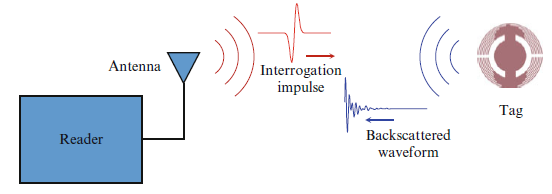
\includegraphics[width=\textwidth]{chipless_architecture} The architecture of chipless RFID systems 
\caption{\label{fig:chipless_architecture}The adopted from \cite[p.18]{chipless}} 
\end{figure}


\subsection{Security and Privacy of RFID systems}

Security and privacy in the healthcare sector is a very important and highly discussed issue. As these are very large issues, which could not be described within a few paragraphs, there will be depicted some examples of threats. In the second section 'Solutions and Methods against Threats' \pageref{solution}, five important recommended countermeasures will be described.

\subsubsection{Security Problems and Threats} \label{problems}
 
As Henrici \cite{henrici} mentions, there exist two fundamental fears about the RFID technology. The first fear concerning marketing purposes, such as creating very detailed customer profiles which lead to a vast amount of information. Secondly, the technology offers the possibility to keep people under surveillance which implies advantages and disadvantages. As an advantage, the patients' life gets more confortable and companies will be more productive. As a negative result, people's privacy is violated and the application's security is not addressed properly.
Aside from the two fears, Henrici describes several risks of RFID systems, such as the ease of disrupting the service which indicates data security and privacy problems. When talking about security, one should distinguish between security of systems and services and the security of data and information. The last point can only be ensured by secure systems \cite{henrici}. 
In the following, some security and privacy risks using RFID technologies will be explained. To start with, one should think of his passport and the data which is stored on it. The new passports have an internal RFID tag which enables readers nearby the passport to read out all data and to copy them as well. As mentioned in section \pageref{tags}, passive RFID tags are cheap, do not have their own power supply and can be read through a nearby reader. So, reading out the passport's data would not be very complex.
Moreover, Henrici mentions product counterfeiting in pharmaceuticals which can cause a lot of harm, like the death of patient's. Nevertheless, the drug market is bound to strong regulations, like for example through the \ac{FDA}. To detect and reduce product counterfeiting, RFID tags need to prove genuineness of original products to patients and should inhibit cloning them.

In his book, Henrici mentions six cases of possible attacks to RFID systems \cite[p.61 ff.]{henrici}. The first attack is called 'Illegitimate reading of data' and describes the possibility of side-channel attacks which use the communication protocol between passive tags and backend systems. As described in section 'RFID backend systems' \pageref{backend}, passive tags are used more often and are less expensive than active tags. Nevertheless, the vulnerability of synchronizing each tag with the backend system through a protocol enables attackers to bypass normal protocols so that they can readout all transmitted data.
The second possible attack, Henrici mentions, is called 'eavesdropping of data'. It is caused by the problem of the public and shared communication channel between readers and tags. Compared to 'illegitimate reading of data', everybody near enough the communication channel is able to eavesdrop the conversation because of the use of passive tags. Particularly the 'forward' channel from reader to tag has a stronger magnetic field than the opposite direction which makes it more easily being eavesdropped than the backed one. 
Thirdly, Henrici declares 'cloning or mimicking of tags' as a third threat. His definition of cloning a tag is restricted to creating an exact logical copy of an item which is not distinguishable from the original tag on the protocol level. There might exist some minor differences like the power consumption or time response but the replica cannot be detected with ordinary readers but only with appropriate equipment. The second term 'mimicking' defines the action of infiltrating incorrect data into the RFID system. To show an example, the location might be used for authentication of items. By mimicking a tag, the location can be manipulated and items might appear where they do not exist in reality.
Fourthly, 'recognition of objects' represents another possible threat of RFID systems. In particular, when persons have been detected, they can be used to explore customer habits. Or, in case of patients who wear implants, these might be recognized and the medical information stored on each implant might be abused. In general, each person who carries objects with affixed RFID tags, like wristwatches, shoes etc. might be recognized by an attacker.
Next, the possibility 'tracking of objects' should be considered carefully since tracking of persons can cause many privacy violations. Henrici distinguishes two types of tracking: The first one is called 'direct mapping' and refers to the tracking of RFID wristwatches or glasses. 'Direct mapping' is only possible when the distance between detector and tag is short and the do not exist many tags in one place. Failing that, other items might be tracked by detecting their constellations to each other. These constellations can lead to unwanted creation of movement profiles and the abuse of infrastructure for surveillance by a totalitarian government.
Lastly, Henrici defines the threat of 'causing malfunction' which means that attackers (after having abused one of the above mentioned possibilities) are able to render RFID system malfunctioning. This malfuncionting can be revealed by physical destruction or chemical treatment of tags.  

\subsubsection{Solutions and Methods against Threats} \label{solution}

First of all, data security should always be maintained by the RFID system. But what are the exact countermeasures to prevent an attack on an existing RFID system? When Henrici \cite[p.64 ff.]{henrici} talks about solutions and methods against security threats, he calls them 'Goals of Security and Privacy'. In his book, these goals refer to the possible attacks or threats mentioned in section 'Security Problems and Threats' \pageref{problems}. In the following, the countermeasures will be explained. 
'Illegitimate reading of data' can be prevented by controlling data access and ensuring data integrity in RFID systems. False data should be infiltrated because of illegitimate access.
'Eavesdropping of data' can be coped with implementing means for detection and recovering so that the system should keep running even if attackers try to put it out of service. Besides, the integrity of system should always be kept. Another strategy preventing eavesdropping is to maintain data security. Henrici defines a 'good' RFID system to be able to cope with illegitimate reading of data and to treat all the data confidentially.
'Cloning or mimicking of tags' which can be compared to counterfeiting can be prevented by using authenticity mechanisms to identify specific tags. Therefore, RFID tags that can prove their own authenticity should be preferred.
Unwanted 'recognition of objects' can be avoided by developing technical models that provide suitable trade-off of functions. If a function is not wanted by the user, e.g. to allow everyone in the surroundings to read out all RFID attached object, he can adjust this by defining different user roles and rights.

Regarding the realization of the above mentioned goals, there exist many challenges which have to be faced. Henrici \cite[p.66 ff.]{henrici} describes four general challenges which will be explained in the following paragraph. 
First of all, since there are different parties, like e.g. logistic companies and customers which have different needs, the developer has to meet all of their requirements. For instance, the different user needs might be realized by developing different views which depend on the particular user role.
Secondly, developing a secure RFID system is a multidisciplinary challenge \cite{henrici} including six different departments: Computer science (designing communication protocols and the middleware), electrical engineering (realizing the required functionality in hardware and physical layer of communication between tags and readers), mathematics (developing basic cryptographic primitives and theory of probabilities for different areas), economics (adapting the application's constraints imposed by laws of market and assessing real world applicability of approaches), social sciences (including user's requirements, such as privacy and usability) and law (maintaining a legislative basis among people and organizations).
Thirdly, there are more requirements to be faced than 'only' security and privacy, such as low costs or coping with few capabilities and resources. Besides, the enrollment of an RFID system, e.g. in a hospital with many distinctive departments, leads to an inter-organizational operation. To implement this inter-organizational operation, several standards have to be integrated. 
Last but not least, additional requirements have to be considered: Scalability of the system, dependability, low complexity of system, robustness, transparency and usability etc. Henrici claims, that the safeguards should not limit the read range and the speed of reading. Moreover, when using cryptographic primitives, migration paths should be considered.  

\subsection{State of the Art}

There exist many companies which develop \ac{RFID} solutions and applications. In this paragraph, three important medical companies which provide RFID solutions, will be presented.

\subsubsection{Dipole Company}

To start with the first company, in the following, the spanish company 'Dipole' \cite{dipole} will be depicted. 'Dipole RFID' was found in Barcelona 20 years ago with the aim of developing systems for intelligent identification, data capture and systems integration. In their product scope, Dipole provides three main products. The first product contains RFID as well as \ac{NFC} solutions which should improve optimizing processes, realizing industry 4.0 and the \ac{IoT}. The second product consists in manufacturing RFID tags to measure the according user needs of Dipole's users. The third product is composed of consulting services, RFID software and systems integration.
In their section 'RFID Hospital and Health', Dipole mentions some use cases for their RFID solutions. To give an example, the correct administration of banked blood can be controlled by using RFID tags. Or, when product stock or termination date of medication and drugs in a hospital have to be observed, RFID tags provide a simple and large-scale use instead of controlling the stock manually (which also brings the risk of human errors). For broader use in hospitals, such as managing whole buildings and improving their workflows, RFID solutions should be considered as well. There exist many hospitals which administrate their workflows with paper-based solutions. As a consequence, the processes are getting very slow and data is duplicated. Furthermore, the communication between several departments is flawed and causes further problems.
Another health service, provided by Dipole, is the 'Traceability of Analysis'. In a hospital or a healthcare institution, there are many processes which embody information about clinical analysis, blood tests and blood preservation. These information are very important for patient's diagnosis and treatment. In a laboratory, all tissue samples are stored and several cultivation processes have to be controlled. To increase efficiency of these processes, establishing a RFID system to track and identify all samples correctly would be a useful solution.
When it comes to the management of buildings and workflows, the asset tracking forms an important part. Dipole distinguishes two different classifications of assets: \ac{RTI} and products of high value, e.g. elements from the IT and mobile machines. The second type of elements needs specific control in real-time. For an appropriate tracking of IT elements it should be possible to locate each item in a global and detail view to be sure that it is settled in the correct place and under the right conditions, such as the correct temperature or low air humidity.
Another use case is guaranteeing the correct dosage of medication to patients which is very important for patient's health and and the work of nursing staff. To simplify the dosage of medication to each patient, RFID tags can be sticked to the pill cases to ensure the correct distribution in real-time. 
Concerning the management of patients, it is possible to track patients indiviually by wearing bracelets which contain a RFID tag. Currently, the tracking of persons is very controversial because the patient's privacy is offended by enabling his persecution. On the other side, RFID bracelets enable to register patient's actions in real-time and ensure their safety. For example, if a patient suffers from epilepsy, it is dificult to predict an epileptic shock. But if he wore a bracelet which constantly synchronizes his health status with the system, doctors would be able to act preventively against such shocks and could minimize his risk to die of his illness.
Not only managing whole buildings is important but also the tracking and control of material in the operating rooms plays a significant role. For instance, in operating room A exists a mobile \ac{CT} whereas operating room B only has set of instruments for surgery. When there is a emergency and the patient needs a CT because the doctor cannot say if he needs the suggested operation but in the operating room B does not exist a CT, it is necessary to detect the next mobile CT rapidly and not to deteriorate the patient's health status. 

\subsubsection{Cardinal Health Inc.} \label{inventory}

Cardinal Health Inc., with its headquarters in Dublin and Ohio, founded 100 years ago,  \cite{cardinal_web} is a global company which provides integrated healthcare services and products. There exist four product fields in the scope of Cardinal Health Inc.: logistics, caring of patients, business solutions, and guidance of patients.
Cardinal Health Inc. provides Inventory Management Solutions \cite{cardinal_video} which are specialized on hospital's inventory. In a promotional video, they quote different types of inventory systems, such as the '2-Bin-Kanban' system which is adapted for low cost items needing right sizing and bulk level. A second inventory system which provides management for low cost items needing oversight at the each level is the 'Barcode' system. For high value implantables and physician preference items, the company advertises RFID as best used technology. In the video \cite{cardinal_video}, they claim that reading RFID tags is fast, e.g. 100 tags can be read in seconds. Moreover, RFID tags implicate ease of use for users and support user's needs very quickly. The physician does not have to care about the data capture of his observation because all RFID tagged items are automatically tracked and the measured data is captured by backend interfaces which synchronize to other IT systems (like Materials Management System or Billing Systems). In addition to that, automatic data capture avoids redundant data entries, provides errors and saves time.
Another important fact about RFID technology is its accuracy and uniqueness. Cardinal Healthcare Inc. advertises that RFID applications enable automated real-time tracking at a unique item level. Beyond, these applications provide a pro-active management of expired and recalled products. As a result, RFID applications lead to a streamlined workflow in which charges are automatically captured for accurate billing and compliants as well as clinical documentation are supported. 
All in all, Cardinal Health Inc. claims that by using its Inventory Management Solution for hospitals will enable physicians and nurses to focus more on patient care and spend less time on managing supplies  \cite{cardinal_video}.

\subsubsection{Terso Solutions Inc.}

Terso Solutions Inc., formed in 2005 in Madison (Wisconsin, U.S.), is specialized on RFID product development and provides several \ac{RAIN} RFID solutions. RAIN RFID \cite{rainrfid} is a wireless technology which enables the wireless connection of items to the internet. As a global alliance, RAIN RFID promotes the universal adoption of \ac{UHF} RFID technology which can be compared to the WiFi Alliance. RAIN uses a standardized GS1 UHF Gen2 protocol to connect all members (network, software, readers, tags, items) of its solution.
However, Terso Solutions Inc. has developed a solution for Medical Field Inventory Tracking which prevents a wide range of services to hospitals. In a promo \cite{terso_video}, the company shows its solution which connects the RFID technology to medical field by integrating RFID into the medical kit. By using this Medical Field Inventory Tracking, sales can be instantly recorded, field inventories and reverse overstock situations can be run. Besides, automated inventory reporting is possible which brings the side benefit of eliminating shipping costs. Each wrap can be located by the system and the closest needed device is shown. The advantages that accrued are better handled recalls, eliminated overnight shipping demands and reduced expired products. All in all, Terso Solutions Inc. provides two large RFID applications: The 'RFID for Compliance and Product Integrity' and the 'RFID for Compliance and Implant Tracking' which have also been approved for case studies in two hospitals in the U.S.. The first hospital where Terso Solutions Inc. performed its 'TrackCore' case study was the North Kansas City Hospital. RAIN RFID-enabled intelligent cabinets, integrated with TrackCore Inc.'s tissue and implant tracking software as well as the 'TrackCore Operating Room' were tested. Furthermore, 'Jetstream', a cloud-based platform from Terso was proved at 'North Kansas City Hospital'. The second case study was implemented at St. Dominic Hospital. The tested application included Terso's autoated tissue and implant tracking solution using RFID.

\subsubsection{Vizinex RFID}

Vizinex RFID was founded in 2012 and is located in Bethlehem, Pennsylvania, U.S. Specialized on the development of RFID tags, Vizinex provides tracking, security and authentication solutions which are based on the RFID technology. Concerning RFID, the company mentions several use cases of the technology \cite{vizinex} which will be mentioned in the following. Firstly, RFID can be used to detect  counterfeited drugs. Secondly, the company suggests the use of RFID in the medical equipment field by establishing real time locating systems. As an example, hospital staff is able to rapidly locate critical medical devices, defibrillators. As a positive consequence, Vizinex remarks the enhancement of patient's safety and the reduction of investments in equipment which are needed \cite{vizinex}. Another use case is the inventory management (see also Cardinal Health Inc. \pageref{inventory}) and tracking of consumables used in an operation (like for example scalpels, sponges, clamps or surgical equipment). The last point (tracking of consumables in an operation) indicates that after each operation everything can be automatically accounted for. In respect of the use for patients, Vizinex instruct ID cards, wrist or ankle bands and labels which can be attached to patients records. The company declares these identification possibility as a great aid to ensure that the right procedures and medications are applied (see Chapter 1, Internal Communication \pageref{Kap1}). Regarding the possibility of patient tracking, Vizinex brings up patients with afflictions such as Alzheimer's disease which makes it very difficult to live securely alone. For that reason, tracking people which suffer from Alzheimer within a facility can improve and avoid the risks of getting lost or entering an area where these people might harm themselves. In regard to laboratories, Vizinex names the following examples. The RFID technology can be used to track tissue or fluid samples. While samples are moved through various preparation steps there can occur several errors from data entry or mishandling which can be avoided by automatic tracking. Consequently, the samples that arrive at the pathologist for analysis will automatically contain the related patient record. Besides, an indication can be called to the computer screen to ensure the proper association of the sample with the patient. 
As another example, Vizinex depict RFID uses for the discovery of drugs. Especially valuable assets are difficult to inventory but it is essential to do this with a high level of accuracy.
All in all, there exist many use cases for the RFID technology. Nevertheless, the use of this technology brings up some concern related to the confidentiality of medical information \cite{vizinex}. Vizinex calls RFID tags 'licence plates' for the items they tag because only the identification number is contained on the tag whereas all 'human readable' information (such as the asset, drug, tissue sample or patient) resides in a database. The FDA highly recommends the external storage of confidential and private patient data and proposes an outline of three components for ensuring medical information security \cite{vizinex}. First of all, all information should be kept confidential. Secondly, the data should be accurate and complete. Thirdly, the data should be available and accessible. To realize the third component, the information should be store on a computer based system. 
By maintaining these provisions, data entry errors will be reduced, work and information flows will be automated, asset and consumable inventories will be improved and the association of treatment plans with patients will be improved. % Externe Datei einbinden
\chapter{Development of Medication Tracking Application}
\label{Kap3}

%talking about platforms in general, to get a common understanding 
\section{Used platforms and technologies} \label{platforms}

This chapter focusses on explaining the used technologies and frameworks for developping the mobile RFID application. In the following, the framework 'Nativescript' which can be used for native mobile development will be explained. After that, a further section will discuss the technology of NoSQL and will compare it to SQL database technology. This section will also depict MongoDB, a document store. Finally, the Impinj RFID reader will be presented. In the last section \pageref{app_development} of this chapter the challenges as well as the user scenarios will be shown. 

\subsection{Native Development with NativeScript} 

There exist several ways to create a mobile application. But the challenge is to develop a consistent solution for the existing systems, like e.g. Android or iOS.
To face the challenge of developing both an Android and iOS application, one has to think of the usage of web development technologies, like for example HTML5, CSS and Javascript. These technologies provide the advantage of using the access to browser/internet  connection.

\subsubsection{NativeScript Sidekick}

\begin{figure}
\centering
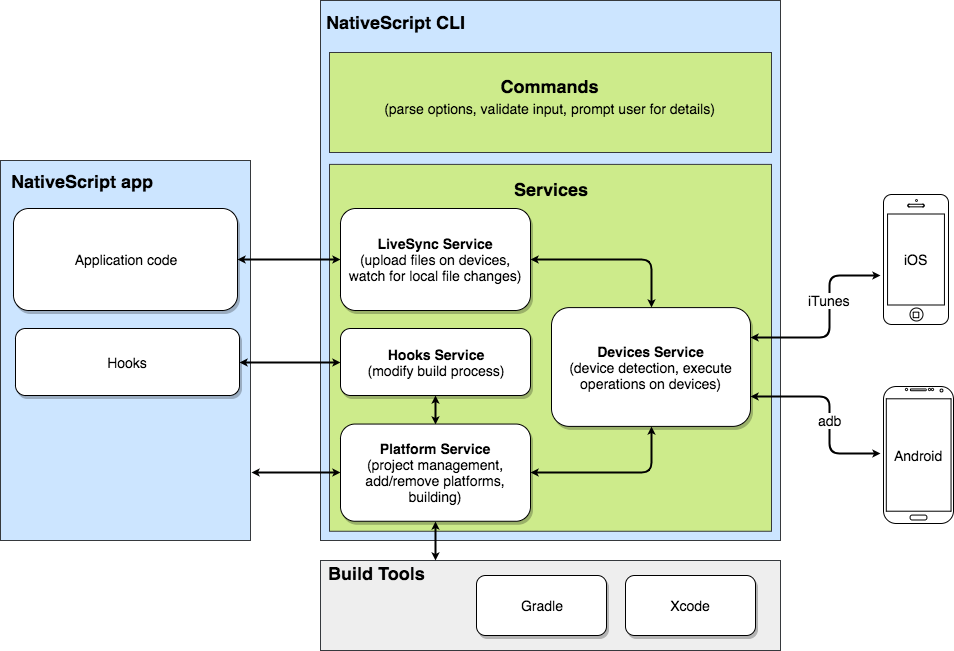
\includegraphics[width=\textwidth]{nativescript_functionality} 
\caption{\label{fig:nsarchitecture}The architecture of NativeScript Applications, adopted from \cite{nsarchitecture}} 
\end{figure}

editor for writing simultaneously apps at one moment (both for Android and iOS devices)

\subsection{Technology of NoSQL} \label{nosql}

There are many possibilities to store data from application systems. \ac{SQL} can be seen as one of the fundamental database technologies used since the 1980/1990ies \cite[p.137 ff.]{nosql_meier}. The technology of SQL offers advantages, such as consistency, security and integrity of data, as well as the protection of transactions. On the other side, there come along many disadvantages while using SQL. To give an example, checking the integrity of data in case of a higher amount of data implicates the need of a higher processing power. Furthermore, facing large-scale development, the efficiency and performance of SQL based systems are decreasing. Moreover, the flexibility and data handling demonstrates another challenge when using SQL. Actually, in practice, the performance is often more important than the consistency, e.g. in social media.    

In addition to that, many companies are missing clear concepts of architecture as well as migration strategies for the optimal application of  'post-relational databases'. To make SQL databases more flexible and to solve the above mentioned problems, Meier and Kaufmann discuss 'post-relational databases' \cite[p.187 ff.]{nosql_meier}. These databases provide on the one hand partial extensions to relational database systems, on the other hand they offer complete new concepts and methods. To give an example, Meier and Kaufmann talk about decentral or federated databases which imply that the data is distributed on different locally seperated computers \cite[p.188 ff.]{nosql_meier}. By replicating the whole data pool and fragmenting it into different smaller parts which are distributed on several computers, decentral databases raise the data volume effectively. The fragments are called 'shards' and the concept of fragmentation is called sharding or partitioning \cite[p.188 ff.]{nosql_meier}. By using decentral databases, users only have to consider the logical view of data and not the physical fragments, all operations on the database will be driven by the database system.  
Alongside the decentral databases there are also introduced other 'post-relational databases', such as 'Temporal databases', 'Multi-dimensional databases', 'Object-relational databases', 'Knowledge/deductive databases' and 'Fuzzy databases'.

However, there were some NoSQL database technologies coming up in the past ten years. In 2000, these databases were called 'Web-Scale-Databases' because of the need of data storage systems which should handle with the large amount of data of web services \cite[p.221 ff.]{nosql_meier}.
The term NoSQL can be understood as 'Not only SQL' which signifies extension of the existing SQL functionalities. Some data specialists prefer the context of 'no relational databases' which is controversial because of the use of graph databases which deal with relations between nodes.   
In the next section, some examples for the NoSQL data management will be explained and compared to the usual SQL data management. According to Meier and Kaufmann \cite[p.3 ff.]{nosql_meier}, SQL databases are formed on a relation-based model which contains tables with entries. Furthermore, each entry has attributes which are defined by a validating range. A table is defined by its table name, the attribute's name and an identification key. It can have both a column or row order or none of these. The relational model indicates that every table is a set of random tuples and that the relations between data is realized by using tables. The result of SQL queries are always tables which can be uniquely, minimally identified by their identification or primary key.

In contrast to that, the technology of NoSQL offers more possibilities to store data, like for example in key-value stores, column stores, document stores or graph databases \cite[p.16 ff.]{nosql_meier}. These four types of NoSQL databases are also called 'Core-NoSQL-Models'. Besides, other NoSQL database models like object databases, \ac{XML} databases or grid databases are defined as 'Soft NoSQL Models'. 
To give some examples of the 'Core-NoSQL-Models', their fundamental characteristics will be described in the following. The key-value stores (e.g. Cassandra) provide the simplest way to store data by using an identification key and a list of values. Document stores (like e.g. MongoDB \pageref{mongodb}) store the data in form of structured text data like \ac{JSON} or XML. In contrast to key-value stores, document stores have a pre-defined structure but are schema-free which means that the data structure can be changed over the time. Graph databases (e.g. Neo4J) introduce a new way to store data: It introduces a graph-based model. Each graph consists of nodes and edges which connect the edges and demonstrate their relations. Each node can have concepts and object. Both, nodes and edges have a label and can contain properties. Each property contains an attribute and a value. The query language for graph databases is called 'Cypher' \cite[p.16 ff.]{nosql_meier} which is a declarative language. Users of Neo4J and other graph databases are able to specify their retrieval query by defining nodes and edges. By evaluating all possible paths (or connections between nodes and edges), the database system calculates all requested patterns.   
Generally, NoSQL technologies are popular for their high availability as well as their protection against system failures by using different replication concepts, e.g. 'Consistent Hashing' \cite[p.11 ff.]{nosql_meier}. In addition, NoSQL is characterized by its vertical and horizontal aligned scalability, its weak or non-existent restrictions concerning schemas and data models. Along, NoSQL databases offers simple data replication and easy access through API \cite[p.221 ff.]{nosql_meier}.  
Edward and Sabharwal discuss the pro and cons of NoSQL technologies in their book \cite[p.17 ff.]{mongodb_edward} which will be given in the next paragraph.
One the one hand, NoSQL offers high scalability, manageability and administration (such as automated repairs, distributed data etc.), low cost and flexible data models. But on the other hand, using NoSQL factors like maturity, limited query capabilities, administration (installing and maintaining solutions) and limited expertise (developer and administrator community are limited).

\paragraph{Document Stores} \label{documentstore}

In the last section, there were introduced some examples of NoSQL databases. This paragraph reveals with the characteristics, advantages and disadvantages of document stores because the deployed database, MongoDB, is a document store. 
Basically, document stores consists of databases, containing collections with documents. Each document can have its own internal structure and is defined by JSON-like files which look like a list of attribute-value-pairs. As a 
On the one hand, like key-value-stores, document stores are schemafree so that users do not have to define a schema for the database. Nevertheless, document stores offer the possibility of structuring the stored data. In addition to that, the structured data will be stored as records which are called documents. Generally, document stored were developed for web services. Thus, they are easily integrable with JavaScript and \ac{HTTP} and easy horizontally scalable. 
On the other hand, as a disadvantage, document stores do not support referential integrity either normalization.
Nevertheless, because of being schemafree, document stores propose high flexibility to store different data (see section Excursus: BIG DATA \pageref{bigdata}). Referring to the flexibility, fragmentation and sharding of an existing data pool can be seen like that. In excess of relations between data, documents do not have any relation to each other but each document contains a closed collection of data in which familiar data can be linked.

\paragraph{Queries (Map and Reduce)}

Document stores are exceptional in that they query in a Map/Reduce procedure which enables the possibility of querying parallel and accelerated. Consecutive, the Map/Reduce procedure will be explained briefly. 
To begin with, the method can be divided into two phases: During the first phase (Map, 'group by'-phase), the data is grouped by criteria. This is realized by a Map-function which asociates for each document an appropriate specific processing by establishing an index (= map) and sending it back. A map can be compared to an associative array with one or multiple key-value-pairs per document.  
After that, in the second phase (Reduce, 'Aggregation'), a Reduce-function (can be compared to SQL statements) returns for each key in the index a row of the Map-Function and aggregates their related values. This second phase is optional.

\paragraph{CAP theorem} \label{CAP}

The \ac{CAP} theorem \cite[p.15 ff.]{mongodb_edward} also known under the name of  'Brewer's Theorem', was developed Eric Brewer in 2000. It describes three important characteristics of a NoSQL database system: Consistency refers to all data which has to remain consistently after every operation. Availability means that the system itself has to be available at any time. Partition tolerance states that every system is working even if is partitioned into groups of independent servers \cite[p.15 ff.]{mongodb_edward}.

\paragraph{ACID vs. BASE}

Concerning the topic of transactions in SQL, Meier and Kaufmann \cite[p.136 ff.]{nosql_meier} mention the \ac{ACID} principle. Atomacity means that a transaction is either performed completely or not. Consistency refers to transactions which cause conviction from one state into another. At this point, Meier and Kaufmann declare a transaction as 'an unit to obtain consistency'. Isolation signifies parallelly run transactions which will produce the same results as single-user environments becaue each transaction is run isolated. The Isolation principle includes the protection from unwanted side-effects. When talking about the isolation of transactions, they can be called 'unit of serializability'. The last principle, durability refers to the different states of databases which have to be maintained until the next transaction. In that case, every transaction can be seen as 'unit of recovery'.

The \ac{BASE} principle which refers to NoSQL technologies says that a consistent state in a distributed database system can take place retartedly. Based on the CAP theorem \pageref{CAP}, BASE signifies that the system is always available and that all states in the systems are soft which means that even if there is no input provided to the system, the state will be changed over time \cite[p.15 ff.]{mongodb_edward}. The last feature of BASE stands for eventually consistency which means that the system will attain consistency in long run provided no input is sent.

When comparing both ACID and BASE, apparently there exist many parallels. 'Atomacity' can be compared to 'Basically Available', 'Consistency' to 'Eventually Consistency', 'Isolation' to 'Soft State'. But one criteria of ACID is not realized within BASE: Durability \cite[p.1 ff.]{mongodb_edward}.

\subsubsection{Characteristics of NoSQL Databases}

A \ac{DBMS} defines a software which describes, stores, queries data independently from an application \cite[p.2 ff.]{nosql_meier}. It consists both of a storing and managing component. The storing component is composed of all data which has to be stored in organizational form and their description. The managing component contains a querying or manipulating language to evaluate data and to change them, such as access control units and an user interface. When it comes to the use of web applications and a heterogeneous data pool in real-time, SQL databases are often not suitable for these problems. In this case, a NoSQL database should be considered. 

\subsubsection{Excursus: BIG DATA} \label{bigdata}

The following section shall only act as additional contextual knowledge paragraph. 
The term 'Big Data' has been emerged during the past 10 years. Due to the enormous data pool, e.g. in social networks or user analysis, which is not easy to manage with usual software tools, new data technologies were needed. As a solution, NoSQL technologies have been arised. Furthermore, Big Data refers to unstructured data which comes from different sources \cite{nosql_meier}. 
Edward and Sabharwal define Big Data as the following: It is a '[...] term used to describe data that has massive volume, comes in a variety of structures and is generated at high velocity. This kind of data poses challenges to the tradtitional \ac{RDBMS} used for storing and processing data. Big Data is paving way for newer approaches of processing and storing data.[...]' \cite[p.1 ff.]{mongodb_edward}. Furthermore, Edward and Sabharwal refer to an explosion of data created by smartphones, social networking sites, in short words from various sources in various formats, such as video, text, speech, log files and images. The type of stored data varies by its 'sector', e.g. retail and whole sale, administrative parts of government, financial services mainly generate text or numerical data (including customer data and transaction information). On the other hand, in the healthcare, manufacturing, media and communication sector especially multimedia as well as image data is produced. To give an example, X-Rays, CT and other scans dominate the storage volumes in healthcare. 
Another important point, when it comes to large amounts of data is the consumation model or the various sources from which data is produced and subsequently consumed \cite[p.6 ff.]{mongodb_edward}. Edward and Sabharwal declare two models: In the old model, few companies produced data and all others (users, clients, etc.) consumed them. But nowadays, they claim that '[...] all of us produce data and all of us consume them [...]' \cite[p.6 ff.]{mongodb_edward}. This creates a new challenge of developing multiple user data models and make the existing data management system more scalable than in the past. 

\paragraph{Velocity, Variety, Volume}

When talking about Big Data, often there come up three descriptive terms: Velocity, Variety and Volume.
Velocity refers to the real-time high-speed evaluation of the upcoming data \cite{nosql_meier},  also known as 'real-time insight' \cite{mongodb_edward}. Edward and Sabharwal describe velocity as 'Data in motion' \cite[p.7 ff.]{mongodb_edward}. Besides, they mention that if data cannot be processed at required speed, it losses its significance. For many companies and organizations, it is very important to process data both when it is moving as well as when it is static. 
Variety means that there are distinct formats of data: structured (e.g. integer, string), semi-structured and unstructured data \cite{nosql_meier}. Edward and Sabharwal describe variety as 'Data in many forms' \cite[p.7 ff.]{mongodb_edward}. As mentioned in the last paragraph, data can vary from simple text files, log files, streaming videos, photos, meter readings, stock ticker data, PDFs and many other unstructured format.   
The last characteristic of Big Data, volume, deals with the high amount of data \cite{nosql_meier}. Edward and Sabharwal describe volume as 'Data in many forms' \cite[p.7 ff.]{mongodb_edward}. They see a reason for the higher volume in businesses becoming more transaction-oriented and the number of transactions is increasing. Moreover, more devices are connected to the internet which increases the size of data.
Calolas et al. refer to challenges like e.g. dealing with tremendious amounts of data, unstructured data (diversity of \ac{OSN}) as well as the complexity to challenge analyzing social networks data \cites{trends_nosql}.

\paragraph{Usage of Big Data}

Edward and Sabharwal depict five large use cases of Big Data which will be explained in the following \cite[p.9 ff.]{mongodb_edward}. Firstly, visibility of data is very important for many companies. For example if data is accessible across departments of a company, it can be readily integrated. This reduces the search and processing time, improves product quality according to present needs \cite[p.9 ff.]{mongodb_edward}. Secondly, discover and analysis information is another use case for large amounts of data. After capturing detailed data, e.g. of inventories, employees or customers, new information or patterns will be discovered and analyzed. The captured information and knowledge can be used to improve processes and performance of companies \cite[p.9 ff.]{mongodb_edward}. Thirdly, segmentation and customizations can be effected by means of using Big Data. To give an example, the segmentation of customers is based on various parameters and can aid in targeted marketing campaigns or tailoring of products to suit the needs of customers \cite[p.9 ff.]{mongodb_edward}. Fourthly, Big Data can aid, improve or automize decision making by using Big Data analytics which can minimize risks and uncover valuable insights. Lastly, Big Data can strengthen innovations in existing products by using data gathered for actual products \cite[p.9 ff.]{mongodb_edward}.    

\paragraph{Big Data challenges}

The issue 'Big Data' not only offers many possibilities or use cases, but also faces many challenges \cite[p.11 ff.]{mongodb_edward} which will be discussed in the consecutive paragraph. To start with, Edward and Sabharwal indicate policies and procedures which can constrain the use of Big Data. They refer to data privacy, security, intellectual property of organizations. Furthermore, in order to comply with various statutory and legal requirements, Big Data has to face the challenge of data handling, which includes issues around ownership and liabilities around data. In second place, the access to data has to be controlled precisely. Since some data might be available to third parties, the gaining access poses a legal, contractual challenge. After that, in order to handle Big Data, new tools as well as technologies have to be built specifically. Moreover, there might exist legacy systems in several organizations or companies which have to deal with Big Data. Besides, there exists a lack of experienced resources in these newer technologies which is also a challenge to.
Most of the legacy systems are designed to work with structured data \cite[p.11 ff.]{mongodb_edward}. Since legacy systems are created to perform fast queries and analysis on tables and columns, they cannot be used to hold or process Big Data (which contains unstructured data). Another important point is the data storage for Big Data. Currently, in many companies, data is stored on big servers (using \ac{NAS} or \ac{SAN} systems) \cite[p.11 ff.]{mongodb_edward}. With the increasing data, the server size and backend storage size has to be increased. 
Lastly, when handling with Big Data, data processing is very important . Usual algorithms in legacy systems are designed to work with structured data and are limited by data size. Therefore, legacy systems are not capable of handling processing of unstructured data, high volumes of data, speed etc. To capture value from Big Data, the deployment of newer technologies are needed. 

\paragraph{Big Data technologies}

Edward and Sabharwal propose several ways of implementing Big Data technologies \cite[p.12 ff.]{mongodb_edward} which will be depicted in this paragraph. To begin with, Big Data needs new storage and processing technologies which are designed for large, unstructured data. After that, other technologies like parallel processing, clustering are emerging in order to handle Big Data. Additionally, large grid environments, high connectivity and high throughput offer new fields for software developer and data scientists. Finally, cloud computing and scale-out architectures have been arised during the last years.

\subsubsection{Use case of NoSQL Databases: 'Socii System'}

To give an example of the use of NoSQL technologies, the next section will focus on explaining a developed system 'Socii'. 'Socii' was developed from Jroge Daniel Calolas, Alda Lopes Gancarski and Pedro Rangel Henriques. In their article 'Online Social Network Analysis Visualization Using Socii' \cite[p.218-228]{trends_nosql}, they describe the several technological challenges they faced during development but also the benefit of this social network analysis and its scientific importance. In short words, 'Socii' is a system which enables the analysis and visualisation of social networks by helping \ac{OSN} users to exploit and understand their own networks through a user friednly interface. During development, Calolas et al. were facing four main principles: simplicity, accessibility, OSN integration and contextual analysis.
One big problem before developing of 'Socii', Calolas et al. mention was the observation of social structures and the analysis of these networks. By establishing 'Socii', the authors Calolas et al. wanted to proprose to fill the gap or struggle that OSN users have in understanding their network. To give an example of these struggles, there were three main topics, Calolas et al. were facing: 'how relationships evolve along the time', 'what role play these friendships within the network' and 'how they can analyze and visualize their networks based on social properties (such as mutual relationships, geographical positions, personal tastes and preferences or hobbies)' \cite{trends_nosql}. 

\paragraph{Structure and flow of data analysis and visualization systems}

When introducing 'Socii' as an social analysis tool, Calolas et al. also talk about several tasks and steps during the process of data analysis and visualization systems. Firstly, data has to be extracted (through APIs, web crawlers and web scrapper. Secondly, data is achieved which requires careful selection of relevant data to store \cite{trends_nosql}. In order to have an efficient system that provides good structure for data analysis, one needs to select the data carefully. In the third step, data is explored by defining of what one user wants to do with the data. Furthermore, during this step, there are two important questions: What are the applications that can be seen for the stored data? How can the system digest and transform data in order to make it useful and interesting for the end user? 
Lastly, in the fourth step, data is visualized which means the kind of presentating or showing the transformed data is chosen by the user. Particularly, the work of the data scientist has a huge impact on the end user. In generals, the data visualization targets a general audience.  
By extension, 'Socii' affirms web availability, OSN's  integration, contextual analysis and being a trade-off for such gains the system performance.

\paragraph{Main functionalities of 'Socii'}

One of the main functionalities of 'Socii' is information extraction and data mining \cite[p.223]{trends_nosql}. These include extracting some user networks form given OSNs by calling web crawler modules which then return the extracted information. After that, an extraction manager sends the extracted data through a simple data mining process in order to data normalized before it is stored in the database (MongoDB). Web crawlers are implemented in Python and the crawling operations are performed using XPath selectors to extract the information that are needed to build the network.
Generally, the main functionalities of 'Socii' amount to OSN contextual netowrk analysis (with relatively low complexity) \cite[p.227]{trends_nosql}. Moreover, 'Socii' intends to integrate data from different OSNs by processing a set of node properties displayed together with the network structure. Roughly, Calolas et al. implemented three features of 'Socii'. To start with, 'configurable, parameterized analysis' enables users to select several metrics upon a given network. Consequently, 'clear, intuitive social graph visualization and interaction' refers to the visual web component of 'Socii' which provides users a set of visual features (coloring, node discovery etc.). Thirdly, 'Socii' offers an 'organized overview upon SNAs and OSN data' which include visual components that aggregate SNAs metrics and OSNs information. Thus, users are able to cross information from both and can derive conclusions from intersecting the information \cite{trends_nosql}. 

\paragraph{Limitations of 'Socii'}

As shown in the last paragraph, 'Socii' offers many features to analyse Big Data especially in social networks. Nevertheless, Calolas et al. depict some limitations and disadvantages which will be explained in the following. 
First of all, there exists a technical and architectural struggle of feeding the system through an extraction pipeline built on top of the web crawlers. This is known and proved by a very slow, limited and error-prone method for data extraction and the authors call it the 'bottleneck' of their built system \cite [p.227]{trends_nosql}. 

\paragraph{Future outlook of 'Socii'}

According to Calolas et al., 'Socii's implementation should be completed to work with other OSN's. Furthermore, it can be extended to perform evaluation and validation of system with users having accounts in several OSNs and several profiles. 

\subsubsection{NoSQL Technology: MongoDB}\label{mongodb}

As mentioned in section Document Store \pageref{documentstore}, this type of NoSQL database provides high availability, scalability and partitioning options \cite[p.25 ff.]{mongodb_edward}. Nevertheless, there are some disavantages when using MongoDB or any other document stores: For instance, both consistency and transactions are not supported. 
In contrast to relational databases, MongoDB does not consist of tables and rows, but of collections containing documents which make it both flexible and scalable \cite[p.25 ff.]{mongodb_edward}. Collections can be compared to tables in SQL but are schemaless. Instead of having one unique schema within the same collection, every document can have its own set of fields, and common fields can store different values across documents.  
All data is stored in \ac{BSON} documents which assures that related data is placed all together in one place. BSON documents are JSON documents in binary-encoded format. It is the extended form of the JSON data model and is fast, high traversible and lightweight \cite[p.31 ff.]{mongodb_edward}. Moreover, JSON/BSON documents contain schema-less models. Each documents stores data as key-value pairs, where the value can be left blank (see above, disadvantage of consistency). Thus, users of MongoDB have to ensure and check the consistency of their data when adding new data.

One characteristic of MongoDB is the _ID (key) which can be compared to the label or name of a colum in RDBMS. If not explicitely specified by the user, a unique value is automatically generated and assigned  to it by MongoDB. Basically, the key value is immutable and can be of any data type except arrays \cite[p.31 ff.]{mongodb_edward}.
Queries in a MongoDB database use the keys (_ID) in documents which makes it possible to query documents spread across multiple servers. 
MongoDB uses primary-secondary replication, where the primary replication accepts the write requests. To be more precisely, if the write performance needs to be improved, the mechanism of sharding can be used. Sharding means that data will be split across multiple machines which are enabled to update different parts of datasets \cite[p.25 ff.]{mongodb_edward}. Besides, this mechanism is automatic in MongoDB, so that as more machines are added, the data is distributed automatically.

\paragraph{Limitations and possibilities of MongoDB}

There are many advantages and disadvantages, limitatiions and possibilities when using MongoDB. The following paragraph will discuss these and give some examples.

Generally, MongoDB offers many features which MySQL does not. To give an example, MongoDB supports secondary indexes, atomic updates at a per document level. Additionally, queries can be executed by using query documents. Furthermore, MongoDB provides replica sets which are based on master-slave replication with automated failover. After that, MongoDB provides a built-in horizontal scaling. Finally, MongoDB can be run everywhere (e.g. on Cloud, \ac{VM}, servers etc.) because it is written in C++. 

Another feature of MongoDB are 'Capped Collections' which store documents in the inserted order. When the capped collection reaches its storage limit, documents will be deleted from the collection in the inserted order (analogous to \ac{FIFO} principle). Capped collections are often used for log files in order to get these automatically truncated after a certain size. In the end, capped collections guarantee preservation order data in the insertion order \cite[p.31 ff.]{mongodb_edward}.

On the other hand, in contrast to relational databases like MySQL, MongoDB does neither support JOINs nor fully generalized transactions \cite[p.25 ff.]{mongodb_edward}. Secondly, when using MMAPv1 as storage engine, the used space is too large because its data directory files are larger than the database's actual data \cite[p.226 ff.]{mongodb_edward}. For that reason, it is recommended to use MongoDB's WiredTiger storage engine which compresses all files and reduces the storage size by 50\%. Moreover, once a collection is dropped diskspace is automatically reclaimed (unlike MMAPv1 engine).
Thirdly, when using MongoDB BSON documents, their usage is limited the size, nested depth and field limits of the specific document \cite[p.228 ff.]{mongodb_edward}. After that, namespaces as well as indexes are limited, for instance the maximum size of indexed items has to be1024 bytes. The number of indexes per collection must not exceed 64 indexes. Moreover, the usage of sharding is limited \cite[p.230 ff.]{mongodb_edward}. Therefore, if shards were implemented too late, a slowdown of servers is caused because splitting and migration of chunks takes time and resources. Thus, Edward and Sabharwal  recommend to shard a collection before reaching 256 \ac{GB}. 
Next, when using MongoDB, there exist some security limitations because the database does not provide authentication by default. This enables every user which is connected to the database server, to read, change, add and delete data. In addition to that, the connections to and from MongoDB are not encrypted by default. Therefore, when starting the database server on a public network, it is recommended to use encrypted communications. Therefore, Edward and Sabharwal propose the SSL-supported build of MongoDB (which is available as 64-bit version) \cite[p.230 ff.]{mongodb_edward}. What is more, using MongoDB implicates write and read limitations, such as case-sensitive queries and type-sensitive fields since there is no enforced schema \cite[p.231 ff.]{mongodb_edward}. For instance, users have to ensure the correctly used type when adding new data. By the same, replica sets which can be used to ensure data redundancy, are limited by the number of the members in every set. When using such replica set, one member acts as a primary member whereas the rest acts like secondary members (a node needs the majority of votes to become primary).

All in all, MongoDB provides many possibilities but also limitations. Generally, it should be clarified that MongoDB is neither adequate to be used in a highly transactional system nor in business intelligence applications where issue-specific databases shall generate highly optimized queries. Finally, it should not be used in applications requiring complex SQL queries. Instead, it is recommended to store high amounts of data and to ensure its availability at any time. 



\paragraph{MongoDB: Best Practices}

\subsection{Impinj RFID Lector and Antenna}

\subsubsection{General Information}

\subsubsection{Examples}

%
% talking about application, more details
%
\section{Application development} \label{app_development}

\subsection{Challenges during development}

Mongodb integration within nativescript application 
--> with Node JS package installer 
but synchronization with data from Mongodb was difficult

Real-time synchronization of mobile application with MongoDB server was difficult. Firstly, HTTP Request/Response was implemented to connect the mobile device with the RFID reader and the database. But only one device was enabled to connect to the server. Thus, another solution had to be considered. Finally, a Socket.IO connection was implemented to both server and client. Socket.IO enables two-way data synchronization and cannot be compared to HTTP Request/Response. Furthermore, with Socket.IO, it was possible to run the application on various mobile devices without any complication. 

\subsection{Progress of development}

\subsubsection{User Scenario}

The following two images show the start page and the item information page of the developed application. 

\begin{figure}
\centering
\subfigure[Start page of application]{\label{fig:a}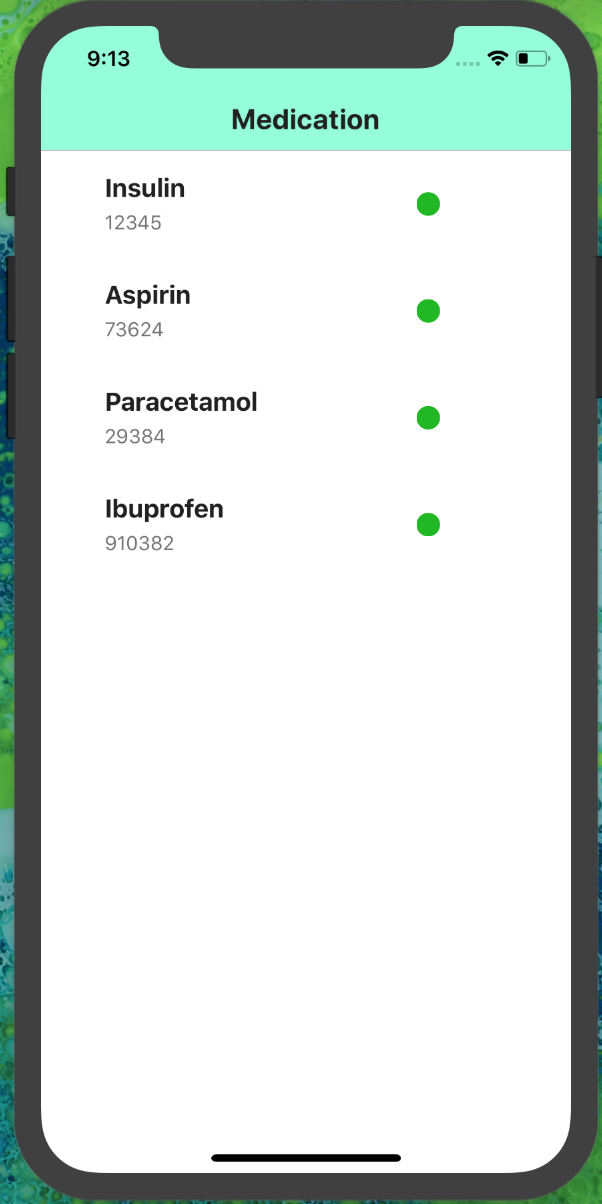
\includegraphics[width=6cm, height=12cm]{Mainview}}
\subfigure[Item information page]{\label{fig:b}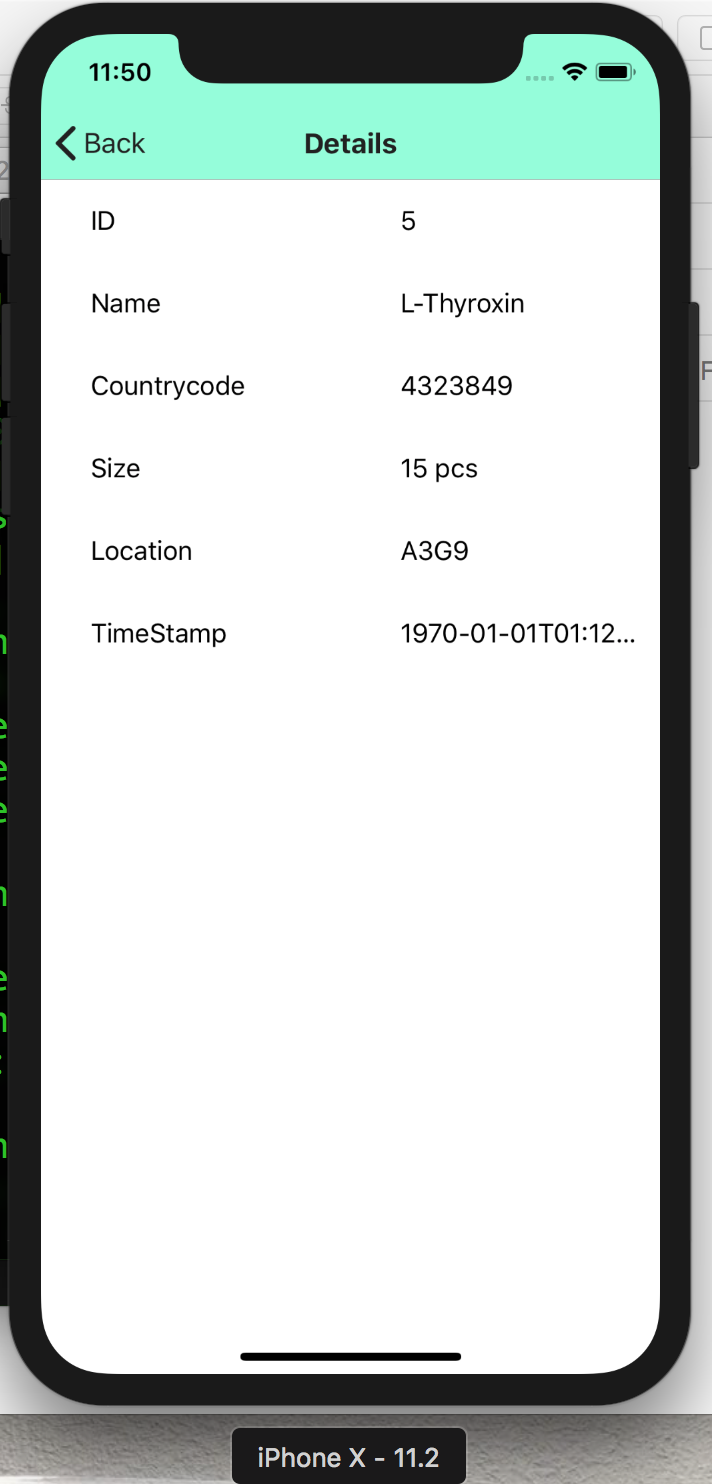
\includegraphics[width=6cm, height=12cm]{Detailview}}
\caption{Layout of application, Screenshot of iOS Simulator}
\end{figure}




\subsubsection{Software Architecture}

\begin{figure}
\centering
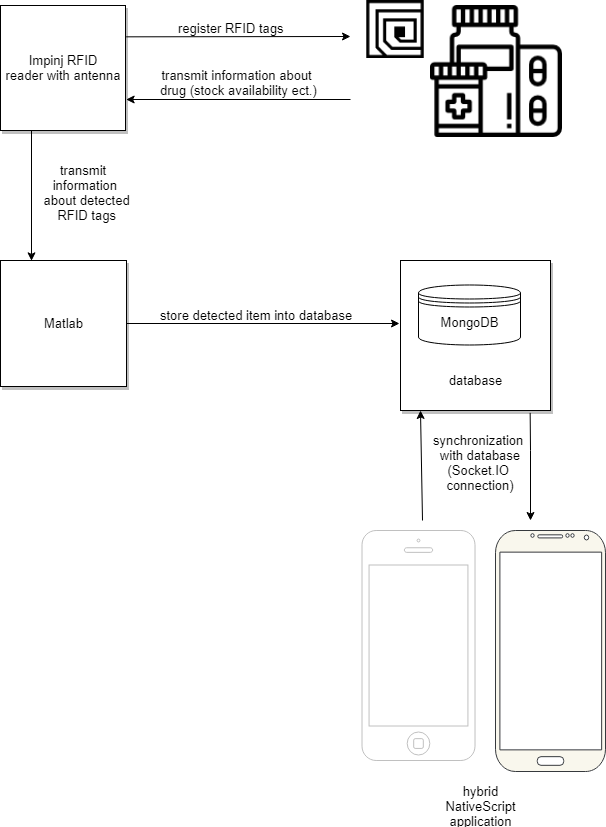
\includegraphics[width=\textwidth]{app_architecture} 
\caption{\label{fig:apparchitecture}The developed system architecture of the mobile RFID application} 
\end{figure}

picture of general software architecture: 
2 antennas, 1 lector (RFID Impinj), Database (MongoDB), GUI: Android and  iOS Application 


\begin{figure}
\centering
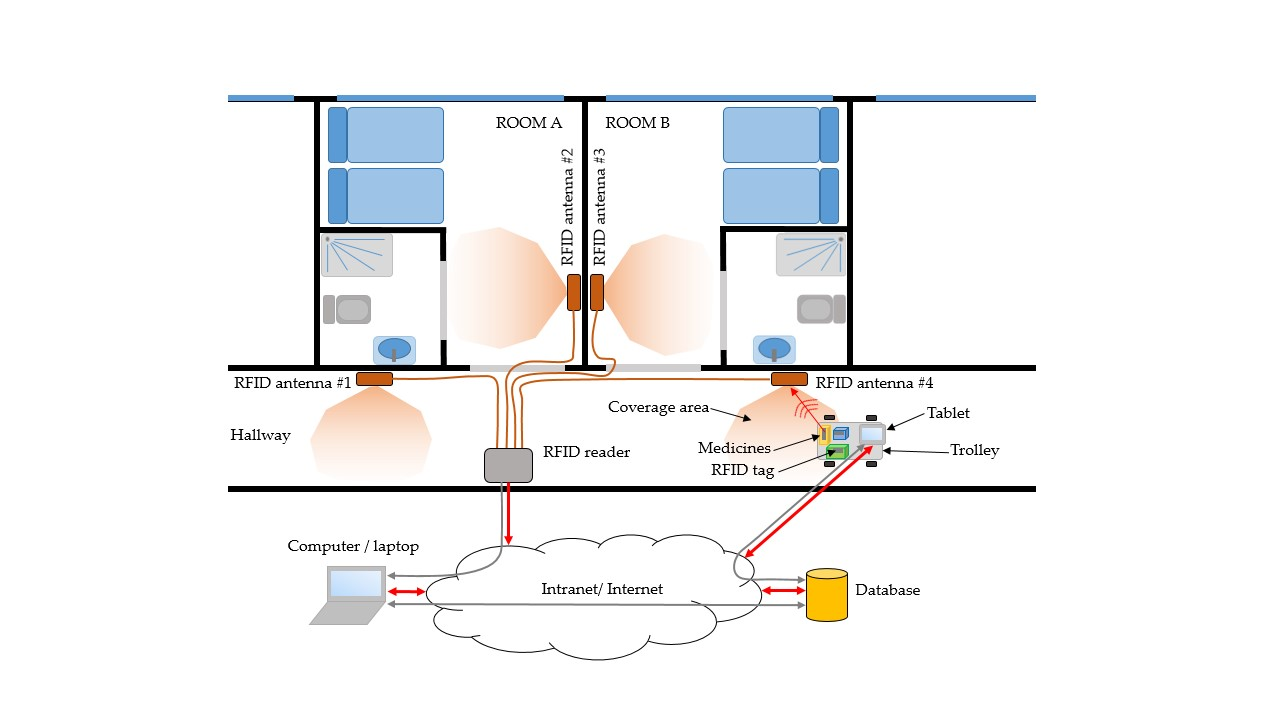
\includegraphics[width=\textwidth]{app_functionality} 
\caption{\label{fig:appfunctionality}Application scenario of RFID application } 
\end{figure}

\subsection{Possibilities of extension}

Henrici \cite[p.121 ff.]{henrici} describes four alternative channels to authenticate and authorized the right tags and to prevent attacks on RFID applications. 
The first possibility of an alternative channel is to use written text to authenticate special operations, for instance on packaging. The master key can be printed on the interior of the product package and is proposed as key recovery mechanism.
Furthermore, optical barcodes can be used together with RFID to ensure identification of items. Especially barcodes attached to each item can be used for general identification of objects. Additionally, RFID tags might be used to assign items of high value.
A third possibility of using side channels is to use optical input, such as photodiodes attached to RFID tags. Each RFID tag can use flashes of light (also called optical channel) to transfer data.   
Lastly, a physical contact channel can also be used alternatively. Compared to smartcards, this methods defends against wireless sabotage or denial of service attacks.


















 
 % Externe Datei einbinden
% ------------------------------------------------------------------

\label{lastpage}

% Neue Seite
\cleardoublepage

% Backmatter mit normalem Zeilenabstand setzen
\singlespacing

% Römische Ziffern für die "Back-Matter", fortlaufend mit "Front-Matter"
\pagenumbering{roman}
\setcounter{page}{\value{frontmatterpage}}

% Abkürzungsverzeichnis
\addchap{\hsmaabbreviations}
% Die längste Abkürzung kann in die eckigen Klammern
% bei \begin{acronym} geschrieben, um einen häßlichen
% Umbruch zu verhindern
\begin{acronym}[WORM]
\acro{RFID}{Radio Frequency Identification}
\acro{NFC}{Near Field Communication}
\acro{IoT}{Internet of Things}
\acro{CT}{Computer Tomograph}
\acro{RTI}{Reusable Transport Items}
\acro{IT}{Information Technology}
\acro{UHF}{Ultra High Frequency}
\acro{RAIN}{RAdio Frequency IdentificatioN}
\acro{HIS}{Hospital Information System}
\acro{RIS}{Radiology Information System}
\acro{LIS}{Laboratory Information System}
\acro{EPC}{Electronic Product Code}
\acro{WORM}{Write Once Read Many}
\acro{WARD}{Wisely Aware RFID Dosage}
\acro{MIMS}{Mobile Intelligent Medical System}
\acro{LF}{Low Frequency}
\acro{HF}{High Frequency}
\acro{UHF}{Ultra High Frequency}
\acro{SSL}{Secure Sockets Layer}
\acro{TLS}{Transport Layer Security}
\acro{FDA}{Federal Drug Administration}
\acro{SMLE}{Single Logical Message Exchange}
\acro{SARS}{Severe Acute Respiratory Syndrome}
\acro{LBMS}{Location-based Medical Service}
\acro{TMUH}{Taipei Medical University Hospital}
\acro{ERP}{Enterprise Resource Planning}
\acro{HL7}{Health Level 7}
\acro{DICOM}{Digital Imaging and Communications in Medicine}
\acro{IoT}{Internet of Things}
\acro{CATS}{Compact Approximator based Tag Searching protocol}
\acro{ITSP}{Iterative Tag Search Protocol}
\acro{CW}{Continuous Wave}
\acro{VHF}{Very High Frequency}
\acro{RCS}{Radio Communication System}
\acro{UWB}{Ultra Wide-Band}
\acro{FMCW}{Frequency-Modulated Continuous Wave}
\acro{SNR}{signal-to-noise}
\acro{TDR}{time-domain reflectometry-based}
\acro{SAW}{surface acoustic wave}
\acro{CMT}{characteristic mode theory}
\acro{SEM}{singularity expansion method}
\acro{TOA}{time of arrival}
\acro{MF}{matched filter}
\acro{SOA}{Service-oriented architecture}
\acro{WLAN}{wireless local area network}
\acro{IrDA}{Infrared Data Association}
\acro{PC}{Personal Computer}
\acro{SOAP}{Simple Object Access Protocol}
\acro{API}{Application's Programming Interface}
\acro{WfMS}{Workflow-Management System}
\acro{ASP}{application-service-provider}
\acro{ESB}{Enterprise Service Bus}
\acro{SWOT}{Strengths Weaknesses Opportunities Threats}
\acro{CEP}{Complex Event Processing}
\acro{SME}{Small and Medium-sized enterprises}
\end{acronym}


% Tabellenverzeichnis erzeugen
\cleardoublepage
\phantomsection
\addcontentsline{toc}{chapter}{\hsmalistoftables}
\listoftables

% Abbildungsverzeichnis erzeugen
\cleardoublepage
\phantomsection
\addcontentsline{toc}{chapter}{\hsmalistoffigures}
\listoffigures

% Listingverzeichnis erzeugen
\cleardoublepage
\phantomsection
\addcontentsline{toc}{chapter}{\hsmalistings}
\lstlistoflistings

% Literaturverzeichnis erzeugen
\begin{flushleft}
\printbibliography
\end{flushleft}

% Index ausgeben. Wenn Sie keinen Index haben, entfernen Sie einfach
% diesen Teil.
\cleardoublepage
\phantomsection
\addcontentsline{toc}{chapter}{\hsmaindex}
\printindex

% Anhang. Wenn Sie keinen Anhang haben, entfernen Sie einfach
% diesen Teil.
\appendix
\chapter{First Appendix}

Hier ein Beispiel für einen Anhang. Der Anhang kann genauso in Kapitel und Unterkapitel unterteilt werden, wie die anderen Teile der Arbeit auch.

\chapter{Zweiter Anhang}

Hier noch ein Beispiel für einen Anhang.


\end{document}
